%%%  Ukázkový text a dokumentace stylu pro text závěrečné (bakalářské a diplomové) práce na KI PřF UP v Olomouci
%%%  Copyright (C) 2026 Jesse Sadowý, <jesse.sadowy23@gmail.com>
%%%  Copyright (C) 2026 Jan Konečný, <jan.konecny@upol.cz>


%%  Pro získání PDF souboru dokumentu je třeba tento zdrojový text v
%%  LaTeXu přeložit (dvakrát) programem pdfLaTeX.

%%  V případě použití programu BibLaTeX pro tvorbu seznamu literatury
%%  je poté ještě třeba spustit program Biber s parametrem jméno
%%  souboru zdrojového textu bez přípony a následně opět (dvakrát)
%%  přeložit zdrojový text programem pdfLaTeX.

%%  Postup získání Postscriptového souboru je popsán v dokumentaci.


%%  Třída dokumentu implementující styl pro závěrečnou práci. Vybrané
%%  nepovinné parametry (ostatní v dokumentaci):

%%  'master' pro sazbu diplomové práce, jinak se sází bakalářská práce

%%  'program=kód' pro Váš studijní program/obor (specializaci), kódy
%%  pro diplomovou práci 'infoi' pro Informatiku (Obecná informatika),
%%  'infui' pro Informatiku (Umělá inteligence), 'ainfpst' pro
%%  Aplikovanou informatiku (Počítačové systémy a technologie), 'uinf'
%%  pro Učitelství informatiky pro střední školy, 'binf' pro
%%  Bioinformatiku, 'inf' pro Informatiku (bez specializací) a 'ainf'
%%  pro Aplikovanou informatiku (bez specializací), jinak je výchozí
%%  ainfvs pro Aplikovanou informatiku (Vývoj software), a pro
%%  bakalářskou práci 'infoi' pro Informatiku (Obecná informatika),
%%  'itp' pro Informační technologie v prezenční formě, 'itk' pro
%%  Informační technologie v kombinované formě, 'infv' pro Informatiku
%%  pro vzdělávání, 'binf' pro Bioinfomatiku, 'inf' pro Informatiku
%%  (bez specializací), 'ainfp' pro Aplikovanou informatiku (bez
%%  specializací) v prezenční formě, 'ainfk' pro Aplikovanou
%%  informatiku (bez specializací) v kombinované formě, jinak je
%%  výchozí infpvs pro Informatiku (Programování a vývoj software)

%%  'printversion' pro sazbu verze pro tisk (nebarevné logo a odkazy,
%%  odkazy s uvedením adresy za odkazem, ne odkazy do rejstříku),
%%  jinak verze pro prohlížeč

%%  'biblatex' pro zapnutí podpory pro sazbu bibliografie pomocí
%%  BibLaTeXu, jinak je výchozí sazba v prostředí thebibliography

%%  'language=jazyk' pro jazyk práce, jazyky english pro anglický,
%%  slovak pro slovenský, jinak je výchozí czech pro český

%%  'font=sans' pro bezpatkový font (Iwona Light), jinak je výchozí
%%  serif pro patkový (Latin Modern)

%%  'figures, tables, theorems a sourcecodes' pro sazbu seznamu
%%  obrázků, tabulek, vět a zdrojových kódů, jinak při =false se
%%  nesází (u theorems a sourcecodes výchozí)

\documentclass[
%  master,
   program=itk,
%  printversion,
   biblatex,
%  language=english,
%  font=sans,
   figures=true,
   tables=true,
%  theorems,
%  sourcecodes,
   glossaries,
   index
]{kidiplom}

%% Informace pro úvodní strany. V jazyku práce (pokud není v komentáři
%% uvedeno česky) a anglicky. Uveďte všechny, u kterých není v
%% komentáři uvedeno, že jsou volitelné. Při neuvedení se použijí
%% výchozí texty. Text pro jiný než nastavený jazyk práce (nepovinným
%% parametrem language makra \documentclass, výchozí český) se zadává
%% použitím makra s uvedením jazyka jako nepovinného parametru.

%% Název práce, česky a anglicky. Měl by se vysázet na jeden řádek.
\title{Procedurální generování dungeonů ve 2D hrách}
\title[english]{Procedural Generation of Dungeons in 2D Games}

%% Volitelný podnázev práce, česky a anglicky. Měl by se vysázet na
%% jeden řádek. Výchozí je prázdný.
\subtitle{Implementace a~srovnání algoritmů v~herním enginu Godot}
\subtitle[english]{Implementation and Comparison of Algorithms in Godot Game Engine}

%% Jméno autora práce. Makro nemá nepovinný parametr pro uvedení
%% jazyka.
\author{Jesse Sadowý}

%% Jméno vedoucího práce (včetně titulů). Makro nemá nepovinný
%% parametr pro uvedení jazyka.
\supervisor{doc. RNDr. Jan Konečný, Ph.D.}

%% Volitelný rok odevzdání práce. Výchozí je aktuální (kalendářní)
%% rok. Makro nemá nepovinný parametr pro uvedení jazyka.
\yearofsubmit{2026}

%% Anotace práce, včetně anglické (obvykle překlad z jazyka
%% práce). Jeden odstavec!
\annotation{Bakalářská práce se zabývá procedurálním generováním dungeonových map ve 2D hrách. Jsou popsány základní principy procedurálního generování obsahu a~vybrané metody tvorby dungeonových struktur. V~herním enginu Godot bylo implementováno a~experimentálně porovnáno pět generovacích algoritmů z~hlediska času generování a~pokrytí mapy průchozím prostorem. Výsledky ukazují výrazné rozdíly mezi metodami a~práce diskutuje vhodnost jednotlivých přístupů pro různé typy herního prostředí.}

\annotation[english]{This bachelor's thesis deals with procedural generation of dungeon maps in 2D games. It describes the basic principles of procedural content generation and selected methods for creating dungeon structures. Five generation algorithms were implemented and experimentally compared in the Godot game engine in terms of generation time and floor coverage. The results show significant differences between the methods, and the thesis discusses the suitability of each approach for different types of game environments.}

%% Klíčová slova práce, včetně anglických. Oddělená (obvykle) středníkem.
\keywords{procedurální generování; dungeon; 2D hry; Godot; herní engine; algoritmus}
\keywords[english]{procedural generation; dungeon; 2D games; Godot; game engine; algorithm}
%% Volitelná specifikace příloh textu práce, i anglicky. Výchozí je
%% 'elektronická data v systému katedry informatiky / electronic data
%% in system of department of computer science'.
\supplements{zdrojový kód aplikace}
\supplements[english]{application source code}

%% Volitelné poděkování. Stručné! Výchozí je prázdné. Makro nemá
%% nepovinný parametr pro uvedení jazyka.
\thanks{Děkuji vedoucímu práce doc. RNDr. Janu Konečnému, Ph.D. za odborné vedení a~cenné připomínky při vypracování této práce.}

%% Nastavení biblatex pro odstranění varování
\ExecuteBibliographyOptions{seconds=true}

%% Cesta k souboru s bibliografií pro její sazbu pomocí BibLaTeXu
%% (zvolenou nepovinným parametrem biblatex makra
%% \documentclass). Použijte pouze při této sazbě, ne při (výchozí)
%% sazbě v prostředí thebibliography.
\bibliography{bibliografie.bib}

%% Další dodatečné styly (balíky) potřebné pro sazbu vlastního textu
%% práce.
\usepackage{longtable}
\usepackage{float}

%% Každá kapitola (\section) začíná na nové stránce
\AddToHook{cmd/section/before}{\clearpage}

\begin{document}
%% Sazba úvodních stran -- titulní, s bibliografickými údaji, s
%% anotací a klíčovými slovy, s poděkováním a prohlášením, s obsahem a
%% se seznamy obrázků, tabulek, vět a zdrojových kódů (pokud jejich
%% sazba není vypnutá).
\maketitle

%% Vlastní text závěrečné práce. Pro povinné závěry, před přílohami,
%% použijte prostředí kiconclusions. Povinná je i příloha s obsahem
%% elektronických dat.

%% -------------------------------------------------------------------

\newcommand{\BibLaTeX}{\textsc{Bib}\LaTeX}

% \noindent\textcolor{red}{\LARGE Upozornění: Následující text
%   dokumentace stylu, vyjma přílohy \ref{sec:ObsahData}, je rozpracovaná
%   a (značně) neúplná verze!!!}

\section{Úvod}
Procedurální generování obsahu, neboli \textit{Procedural Content Generation} (PCG), představuje herním vývoji významný přístup, který umožňuje automatizovaně vytvářet části herního světa na základě předem definovaných pravidel a~algoritmů. V~oblasti digitálních her se tento princip uplatňuje zejména tam, kde je žádoucí vysoká variabilita prostředí, znovuhratelnost nebo snížení nároků na ruční tvorbu obsahu. Jednou z~typických oblastí využití je generování dungeonových map, které tvoří důležitou součást 2D her.

Dungeonové mapy kladou na generování specifické požadavky. Nestačí, aby byly pouze náhodné, ale měly by splňovat základní podmínky hratelnosti, jako jsou průchodnost, přiměřené rozložení prostoru a~vhodné rozmístění herních prvků. Volba generovací metody proto výrazně ovlivňuje výsledný vzhled mapy i~herní zážitek hráče.

Cílem práce je představit vybrané metody procedurálního generování dungeonových map ve 2D hrách, analyzovat jejich vlastnosti a~implementovat jejich praktické ukázky v~herním enginu Godot. Součástí práce je návrh systému v~podobě jednoduché hry, který umožní vybrané algoritmy realizovat, vizualizovat a~následně je mezi sebou porovnat. Důraz je kladen jak na teoretické vymezení problematiky, tak na praktickou implementaci a~zhodnocení výsledků.

Práce je rozdělena do pěti hlavních kapitol: teoretické základy PCG a popis vybraných algoritmů generování, návrh a~implementace praktické části, popis naměřených hodnot, diskuse o~metodách a~naměřených výsledcích a~závěr.

\section{Současný stav řešené problematiky}

\subsection{Procedurální generování obsahu ve hrách}

\subsubsection{Vymezení a definice pojmu}
Procedurální generování ve hrách lze vymezit jako algoritmickou tvorbu herního obsahu s~omezeným nebo nepřímým zásahem člověka. Herní obsah zahrnuje široké spektrum prvků, například mapy, úrovně, pravidla, úkoly, zbraně či předměty a jejich vlastnosti. V~závislosti na konkrétním návrhu může ovlivňovat nejen prostorovou strukturu hry, ale také její mechaniky, obtížnost či samotný průběh hraní \cite{Shaker2016}.

V~současnosti je pojem generování obsahu často spojován s~metodami umělé inteligence, tato práce se však zaměřuje výhradně na algoritmické postupy založené na předem definovaných pravidlech.

Pojem hra je v~odborné literatuře obtížné jednoznačně vymezit, protože zahrnuje široké spektrum forem lišících se cíli, pravidly, mírou interaktivity i~použitou platformou. V~kontextu této práce je proto termín hra chápán jako digitální videohra realizovaná v~reálném čase, ve které hráč interaguje s~virtuálním prostředím přes definované herní mechaniky. Práce se zaměřuje především na 2D videohry určené pro osobní počítače, případně další běžné platformy.


\subsubsection{Výhody a nevýhody procedurálního generování}
Procedurální generování obsahu přináší řadu výhod. Mezi hlavní patří vysoká variabilita výsledného obsahu a~podpora znovuhratelnosti, protože každé spuštění produkuje unikátní prostředí. Dalšími výhodami jsou snížení nároků na ruční tvorbu obsahu a~možnost generování rozsáhlých herních světů s~minimálními paměťovými nároky, jak demonstruje například hra Elite (viz podkapitola~\ref{sec:elite}). Parametrizací generátoru lze navíc přizpůsobit výsledné prostředí různým herním situacím nebo obtížnostem \cite{Shaker2016,Linden2014}.

Využití PCG s~sebou však nese také několik významných omezení. Jedním z~hlavních problémů je nižší míra kontroly nad výsledným obsahem. U~ručně navržených úrovní má vývojář plnou kontrolu nad tempem hry, klíčovými momenty, rozmístěním výzev, předmětů či nepřátel. Naproti tomu u~procedurálního generování je výsledná podoba světa závislá na implementovaném algoritmu a~zvolených parametrech. To může vést k~nevyváženým úrovním, nelogickému rozmístění prvků nebo situacím, které jsou příliš jednoduché či naopak extrémně náročné. Vývojář proto musí věnovat značné úsilí návrhu, ladění a~testování generátoru, aby bylo dosaženo uspokojivé kvality výsledného obsahu.

Dalším rizikem je možnost vzniku repetitivního nebo uměle působícího obsahu. I~přestože je obsah generován automaticky a~náhodně, vychází z~omezené množiny předem definovaných pravidel. Pokud není systém navržen dostatečně variabilně, může hráč postupně rozpoznat opakující se vzorce, což může negativně ovlivnit herní zážitek. Tento problém je sice možné minimalizovat vhodným návrhem algoritmu a~důkladným laděním, nicméně zcela eliminovat jej bývá obtížné \cite{Shaker2016}.

\subsubsection{Přístupy k procedurálnímu generování}
PCG lze klasifikovat podle více kritérií, například podle způsobu reakce na hráče nebo podle deterministické či stochastické povahy výstupu.

Nejčastěji se lze v~praxi setkat s~adaptivním či neadaptivním přístupem, a~to vzhledem k~chování hráče. Neadaptivní (statické) generování vytváří obsah bez ohledu na chování hráče a~jeho průběh hrou. Všechny generované struktury vycházejí ze stejných pravidel a~reakce hráče na podněty neovlivní výsledek. Naopak adaptivní generování pracuje s~informacemi o~hráči. Systém může sledovat úspěšnost hráče, rychlost reakcí, délku průchodu úrovní, využívané herní prvky nebo způsob řešení situací a~na základě těchto dat dále upravovat generovaný obsah.

Dalším důležitým rozdělením je deterministický a~stochastický přístup. Deterministické generování vychází z~pevně daných počátečních hodnot, například seed, což je textová nebo číselná hodnota, která je výchozím bodem pro generátor a~určuje počáteční podmínky algoritmu, podle kterých je následně obsah generován. Při stejném vstupu vždy produkuje stejný výstup. Tento přístup umožňuje reprodukovatelnost výsledků, což je výhodné například při testování nebo sdílení konkrétních map mezi hráči. Stochastické generování naproti tomu pracuje s~náhodností bez pevně stanoveného počátečního stavu, takže výsledky se budou lišit i~při opakovaném spuštění algoritmu.

Z~hlediska procesu generování lze rozlišit konstruktivní metody a~přístup označovaný jako generate-and-test. Konstruktivní metody vytvářejí obsah postupně podle předem definovaných pravidel. Každý krok generování přímo přispívá k~vytvoření výsledné struktury. Naproti tomu metoda generate-and-test nejprve vytvoří potenciální řešení, které je následně ověřeno podle stanovených kritérií. Pokud výsledek nevyhovuje, proces se opakuje. Tento přístup může být výpočetně náročnější, ale umožňuje lépe kontrolovat výsledné vlastnosti mapy.

V~literatuře se rovněž objevuje pojem smíšené autorství (mixed-authorship), kdy se na tvorbě obsahu podílí jak algoritmus, tak člověk. Systém může například generovat návrhy úrovní, které následně autor upravuje, případně může reagovat na částečně ručně vytvořenou strukturu.

Plně automatická generace probíhá bez zásahu člověka během samotného vytváření obsahu. Algoritmus pracuje pouze na základě vstupních parametrů. Tento způsob je typický zejména pro roguelike hry a~další tituly, u~nichž je cílem vysoká variabilita jednotlivých průchodů \cite{Shaker2016}.

\subsection{Historický vývoj procedurálního generování ve hrách}
Počátky procedurálního generování sahají již do 70. let 20. století, kdy byl výpočetní výkon i~dostupná operační paměť velmi omezené. Tyto limity výrazně ovlivnily množství ručně vytvářeného obsahu, a~vývojáři proto hledali způsoby, jak vytvářet variabilní herní prostředí s~minimálními nároky na operační paměť (RAM). Právě z~tohoto důvodu se začaly prosazovat procedurální přístupy \cite{Shaker2016}.

\subsubsection{Beneath Apple Manor}
Jednou z~prvních her, které implementovaly PCG, byla Beneath Apple Manor z~roku 1978. Autorem titulu byl Don Worth a~hru vydalo studio The Software Factory. Hra byla určena především pro počítač Apple II.

Herní prostředí v~Beneath Apple Manor bylo generováno algoritmicky při každém novém spuštění. Rozložení místností, chodeb ani jednotlivých herních prvků či nepřátel nebylo nikdy zcela totožné, a~právě tím byla hra přívětivá pro znovuhratelnost. Cílem hry bylo získat zlaté jablko a~postup bylo možné ukládat, takže po smrti hráče se načetla uložená úroveň znovu, avšak hráč přišel o~část svých atributů.

Autor hry čerpal inspiraci z~programu Dragon Maze, který rovněž využíval náhodné výpočty ke generování bludišť. Tento princip však dále rozvinul a~navrhl algoritmus vytvářející funkční a~hratelnou strukturu dungeonů složenou z~místností propojených chodbami. Hra navíc umožňovala hráči ovlivnit některé parametry generování, například počet místností na jednotlivých patrech, barevnou variantu zobrazení nebo samotnou obtížnost. Po vytvoření struktury úrovně algoritmus náhodně rozmístil také nepřátele, poklady a~další herní objekty. S~rostoucí hloubkou dungeonů se zároveň zvyšovala obtížnost hry, a~to zejména síla nepřátel.

Použitý algoritmický přístup lze zařadit mezi rané příklady způsobu generování založeného na místnostech a~chodbách, který se později stal jedním ze základních modelů využívaných v~hrách typu roguelike. Beneath Apple Manor tak představuje významný historický příklad využití těchto metod, jehož principy byly dále rozvíjeny v~následujících dekádách \cite{Schuller_2021,enwiki:1260179812}.

\subsubsection{Rogue a žánr roguelike}
Hra Rogue si oproti výše zmíněnému Beneath Apple Manor získala výrazně větší popularitu a~měla zásadní vliv na další vývoj podobných her. Právě podle této hry vznikl podžánr označovaný jako roguelike, z~jehož principů dodnes vychází celá řada titulů.

Roguelike hry bývají typické náhodně generovanými úrovněmi, tahovým systémem, permanentní smrtí postavy (permadeath) a~zpravidla i~vyšší obtížností. Náhodné generování zde neplní pouze technickou funkci, ale představuje zásadní designový prvek, který podporuje průzkum, strategické rozhodování i~adaptaci hráče na proměnlivé prostředí.

Hra vyšla v~roce 1980 a~jejími autory jsou Michael Toy, Glenn Wichman a~Ken Arnold. Titul původně vznikl pro unixové systémy a~zobrazoval herní svět pomocí ASCII znaků v~textovém terminálu. Jednotlivé prvky prostředí byly reprezentovány různými symboly, například hráč symbolem~@, stěny znakem~\#, nepřátelé písmeny abecedy. Tento způsob zobrazení nebyl pouze důsledkem technických omezení tehdejšího výpočetního výkonu, ale umožňoval poměrně flexibilní práci s~herním světem a~jeho generováním.

Rogue výrazně zpopularizovalo princip permanentní smrti. Postup hrou nebylo možné ukládat a~jakmile hráč zemřel, musel začít zcela od začátku. Hráči tak zůstávaly pouze nabyté zkušenosti a~znalost herních mechanik. Smrt zde proto nepředstavovala pouze neúspěch, ale také nedílnou součást učení se hernímu systému.

Cílem celé hry je najít Amulet of Yendor, který se nachází v~nejhlubším patře dungeonů, a~následně se vrátit zpět na povrch. Dungeon obsahuje několik pater (tradičně 26) a~každé z~nich je generováno procedurálně. Patra se skládají z~místností propojených chodbami a~jejich rozložení se při každém novém průchodu mění. Náhodně jsou rozmístěni také nepřátelé, pasti, poklady, zbraně a~další předměty.

Prvek náhody se projevuje i~ve vlastnostech předmětů. Například lektvary, svitky či prsteny mají při každé nové hře odlišné označení a~jejich účinek není hráči předem znám. I~pokud hráč nalezne stejný typ předmětu jako v~předchozí hře, jeho vlastnosti se mohou lišit. Tím je posílena nejistota a~nutnost experimentování.

Kombinace procedurálně generovaných úrovní a~permanentní smrti zajišťuje, že každý průchod hrou je unikátní. Hráč se tak nemůže spoléhat na zapamatování konkrétní mapy, ale musí se přizpůsobovat aktuálně vygenerovaným podmínkám. Právě tento princip se stal jedním ze základních stavebních kamenů celého roguelike žánru \cite{PCGRogue,enwiki:1337873899}.

\subsubsection{Elite}
\label{sec:elite}

Dalším významným titulem využívajícím procedurální generování je hra Elite z~roku 1984, kterou vytvořili David Braben a~Ian Bell. Na rozdíl od předchozích her se nejedná o~dungeon, ale o~vesmírný simulátor obchodování a~soubojů. Přesto je Elite z~hlediska procedurálního generování velmi důležitým milníkem.

Hra byla původně vydána pro počítač BBC Micro, který disponoval velmi omezenou pamětí. Z~tohoto důvodu nebylo možné ukládat rozsáhlý herní svět přímo v~paměti. Vývojáři proto zvolili přístup, kdy byl herní svět generován algoritmicky na základě předem definovaného číselného základu. Pomocí tohoto deterministického postupu bylo možné při každém spuštění znovu vytvořit stejnou galaxii bez nutnosti jejího explicitního uložení.

Elite obsahovalo osm galaxií a~ každá z~nich zahrnovala stovky hvězdných systémů. Vlastnosti jednotlivých systémů, jako je jejich název, ekonomika, úroveň technologického rozvoje či typ vlády, byly generovány pomocí pseudonáhodných algoritmů. Procedurálně vznikaly také ceny komodit a~další herní parametry.

Tento přístup ukázal, že procedurální generování není omezeno pouze na tvorbu dungeonů nebo jednotlivých úrovní, ale může být využito i~pro vytvoření rozsáhlých herních světů. Elite tak demonstrovalo, že algoritmické generování obsahu představuje efektivní řešení zejména v~podmínkách s~omezeným výpočetním výkonem a~omezenými paměťovými zdroji \cite{EliteWiki}.

\subsection{Generování dungeonů ve 2D hrách}
Dungeonové mapy se typicky skládají z~místností a~chodeb, obsahují jasně definované průchozí a~neprůchozí oblasti a~musí splňovat požadavky na hratelnost. Generování takových struktur proto vyžaduje algoritmy, které dokáží zajistit nejen variabilitu výsledku, ale i~splnění základních strukturálních vlastností.

\subsubsection{Požadavky na generování dungeonových map}
Při návrhu algoritmu pro generování dungeonové mapy je nutné zohlednit několik základních požadavků, které vycházejí jak z~technických omezení, tak z~hlediska hratelnosti. Generovaná mapa by neměla být pouze náhodným shlukem místností a~chodeb, ale strukturovaným prostředím, které umožňuje smysluplný průchod.

Jedním ze základních požadavků je průchodnost mapy neboli connectivity. Všechny klíčové části mapy by měly být vzájemně dosažitelné, aby nedocházelo k~izolovaným oblastem bez možnosti přístupu. Tento požadavek je zásadní zejména u~her, kde je cílem projít celou úroveň nebo nalézt konkrétní objekt. Výjimkou jsou hry, ve kterých je neprůchodnost záměrná a~hráč se do izolovaných částí dostane například prokopáním.

Dalším důležitým aspektem je kontrola struktury a~rozložení prostoru. Mapa by měla obsahovat přiměřený poměr otevřených a~uzavřených prostor, vhodnou velikost místností a~dostatečně široké průchody, aby hráč mohl bez problémů projít. Příliš husté nebo naopak příliš prázdné prostředí může negativně ovlivnit hratelnost i~orientaci hráče.

Významným požadavkem je rovněž variabilita výsledků. Opakované spuštění generátoru by mělo vést k~dostatečně odlišným mapám, aby byl zachován prvek znovuhratelnosti. Zároveň je však vhodné, aby generování respektovalo určitá pravidla nebo omezení, která zajistí konzistentní kvalitu výsledku.

Z~technického hlediska je důležitá také výpočetní náročnost algoritmu. Generování by mělo probíhat v~přiměřeném čase a~nemělo by výrazně zatěžovat systém, zejména pokud je realizováno za běhu hry (online generování). U~jednodušších 2D dungeonových her je obvykle možné využít algoritmy s~relativně nízkou časovou složitostí, jelikož požadavky na generování jsou značně nižší.

Možnost nastavit velikost mapy, počet místností, hustotu chodeb nebo další vlastnosti generátoru umožňuje lépe přizpůsobit výsledné prostředí konkrétním požadavkům hry a~usnadňuje testování různých konfigurací \cite{Linden2014,Shaker2016}.

\subsection{Přehled metod generování}
\label{sec:prehledMetod}
Metody generování dungeonových map se liší způsobem konstrukce prostoru, mírou kontroly nad výslednou strukturou, typem generovaného prostředí a~výpočetní náročností. Některé algoritmy vytvářejí mapu postupně přidáváním jednotlivých prvků, jiné pracují s~rozdělováním prostoru nebo s~pravidly aplikovanými na mřížku buněk.

Ve 2D hrách převažují metody založené na náhodném umísťování místností a~jejich následném propojování, rozdělování velkého prostoru na menší části nebo algoritmy založenými na takzvané náhodné procházce. Každý z~těchto přístupů má své výhody i~omezení a~je vhodný pro odlišný typ herního prostředí.

\subsubsection{Náhodné umístění místností a chodeb}
Generování pomocí náhodného umístění místností a~chodeb patří mezi nejpoužívanější a~zároveň nejjednodušší přístupy z~hlediska implementace.

Na mapě se nejprve generují místnosti různých velikostí, obvykle obdélníkového nebo čtvercového tvaru. Během generování se kontroluje, aby se nově vznikající místnost nepřekrývala s~již existujícími. Výsledkem je množina místností reprezentovaných například souřadnicemi a~rozměry. Následně jsou jednotlivé místnosti propojeny pomocí chodeb. Ty bývají realizovány jako jednoduché horizontální a~vertikální průchody spojující středy dvou místností nebo jejich nejbližší body. Častým řešením je také propojení ve tvaru písmene L, kdy jsou dvě místnosti spojeny dvojicí kolmých chodeb.

Pro zajištění průchodnosti mapy a~dosažitelnosti všech místností se často využívají algoritmy z~oblasti teorie grafů. Jedním z~typických řešení je použití minimální kostry grafu (Minimum Spanning Tree), která zaručuje propojení všech místností při minimálním počtu chodeb.

Výhodou této metody je především její jednoduchost. Generované dungeony obvykle obsahují přehledně oddělené místnosti a~srozumitelnou síť propojení. Nevýhodou může být menší variabilita, protože místnosti mají pravidelný tvar a~prostředí tak může působit příliš uniformně. Dalším problémem bývá méně efektivní využití prostoru, kdy mezi jednotlivými místnostmi zůstávají větší nevyužité oblasti. Komplikace může přinášet i~samotné propojování. U~jednodušších implementací může docházet ke kolizím chodeb, nevhodnému křížení nebo ke vzniku příliš dlouhých průchodů.

Z~těchto důvodů bývá metoda často kombinována s~dalšími postupy nebo doplněna o~dodatečná pravidla, která omezují velikosti a~vzájemné vzdálenosti místností, délku chodeb nebo celkové rozložení prostoru \cite{Linden2014,Shaker2016}.

\subsubsection{Binary Space Partitioning}

Metoda Binary Space Partitioning (BSP) patří mezi přístupy založené na systematickém rozdělování prostoru. Celá mapa se nejprve reprezentuje jako jeden velký obdélníkový nebo čtvercový prostor, tedy kořen stromu, který je postupně rozdělován na menší části. Každé rozdělení může probíhat horizontálně nebo vertikálně a~výsledkem je hierarchická struktura podobná binárnímu stromu.

Generování obvykle začíná rozdělením celé mapy na dvě části. Tyto části se dále rekurzivně dělí, dokud nedosáhnou určité minimální velikosti. Každé rozdělení vytváří dva nové uzly ve stromové struktuře. Listové uzly představují konečné oblasti. Takto vzniklá stromová reprezentace umožňuje přehledně uchovávat strukturu rozdělení prostoru.

Ve vzniklých oblastech jsou následně vytvořeny místnosti, jejichž velikost je o~něco menší než velikost dané oblasti. Tím vzniká přirozený prostor mezi místnostmi, který může být využit například pro generování chodeb nebo dalších herních prvků. Místnosti jsou propojovány postupným spojováním sousedních uzlů stromové struktury.

Díky tomuto postupu lze relativně snadno zajistit vzájemnou dosažitelnost všech místností. Zásadní výhodou BSP je dobrá kontrola nad velikostí a~rozmístěním jednotlivých částí mapy. Parametry dělení prostoru umožňují ovlivnit výsledný vzhled prostředí a~předejít situacím, kdy by vznikaly příliš malé nebo naopak příliš velké místnosti.

Nevýhodou této metody může být opět poměrně pravidelný a~místy uniformní vzhled generovaného prostředí, protože výsledná struktura často odráží samotný způsob dělení prostoru. Mapy vytvořené pomocí BSP tak mohou působit méně přirozeně než mapy generované například pomocí Buněčných automatů \cite{Linden2014,Shaker2016}.

\subsubsection{Metoda Náhodné procházky}

Metoda Náhodné procházky, často označovaná také jako Drunkard's Walk, je založena na jednoduchém principu postupného rozšiřování prostoru pomocí pohybu náhodným směrem. Algoritmus začíná na předem dané počáteční pozici na mapě a~v~každém kroku se náhodně přesune do jednoho ze sousedních polí. Směr pohybu je obvykle vybírán ze čtyř základních směrů v~mřížce, tedy nahoru, dolů, doleva nebo doprava.

Při každém kroku je aktuální buňka označena jako průchozí prostor. Postupným opakováním tohoto procesu vzniká síť chodeb a~otevřených oblastí, jejichž tvar závisí na délce a~průběhu Náhodné procházky. Výsledná struktura mapy bývá velmi nepravidelná a~rozdílná při každém generování.

Proces generování obvykle pokračuje na základě předem stanoveného počtu kroků, nebo dokud není dosaženo určitého poměru průchozích buněk. V~některých variantách algoritmu může být použito více nezávislých „chodců“, kteří se po mapě pohybují současně a~vytvářejí tak komplexnější strukturu prostředí.

Výhodou této metody je velmi jednoduchá implementace a~schopnost generovat přirozeně působící struktury. Nevýhodou je naopak menší kontrola nad výsledným tvarem mapy a~obtížnější zajištění rovnoměrného využití prostoru. V~některých případech může docházet k~tomu, že většina průchozích oblastí vzniká v~blízkosti počáteční pozice algoritmu, zatímco jiné části mapy zůstávají téměř nevyužité.

Podobně jako u~Buněčných automatů se tato metoda často používá pro generování prostředí připomínajícího jeskyně \cite{Shaker2016}.


\subsubsection{Buněčné automaty}

Buněčné automaty představují přístup k~procedurálnímu generování založený na aplikaci specifických pravidel na mřížku buněk. Mapa je v~tomto případě reprezentována jako dvourozměrná mřížka, kde každá buňka může být například ve stavu podlaha nebo prázdný prostor. Na začátku generování je mapa obvykle inicializována náhodným rozdělením těchto stavů, což vytváří základní strukturu pro další postup.

Následně se celá mapa prochází a~stav jednotlivých buněk se aktualizuje na základě stavu jejich sousedních buněk. Nejčastěji se používá takzvané Mooreovo sousedství, které zahrnuje osm buněk obklopujících aktuální buňku. Pravidla generování bývají různá. Mohou například určovat, že buňka zůstane průchozí pouze tehdy, pokud má dostatečný počet průchozích sousedů. Buňka zůstane prázdnou, nebo se změní na stěnu, pokud je obklopena větším množstvím prázdného prostoru.

Opakovaným aplikováním těchto pravidel dochází k~postupnému vyhlazování náhodně vytvořené struktury. Izolované buňky nebo malé skupiny buněk se postupně odstraňují a~vznikají větší souvislé oblasti. Výsledkem jsou mapy s~nepravidelnými tvary, které často připomínají přirozené jeskynní systémy.

Výhodou této metody je schopnost generovat organicky působící prostředí s~nepravidelnými tvary, které se liší od klasických dungeonů. V~literatuře je algoritmus popisován jako výpočetně efektivní, protože každý simulační krok prochází mapu v~lineárním čase vzhledem k~počtu buněk. Nevýhodou může být menší kontrola nad přesnou strukturou mapy a~také nutnost dodatečných kroků, které zajistí průchodnost celé mapy. V~implementaci může často docházet k~vytváření izolovaných částí a~v~některých případech je proto nutné je zcela odstranit nebo dodatečně propojit, což negativně ovlivňuje složitost algoritmu \cite{Linden2014,Shaker2016}.

\subsubsection{Metoda Bludiště}

Metody generování bludišť vytvářejí struktury tvořené převážně úzkými chodbami, které tvoří souvislou síť průchodů. Mapa je v~tomto případě obvykle reprezentována jako mřížka buněk oddělených stěnami. Samotné generování spočívá v~postupném odstraňování těchto stěn tak, aby vznikly propojené průchody.

Tyto algoritmy často vycházejí z~principů grafových algoritmů, například prohledávání do hloubky (Depth-First Search) s~návratem (Backtracking) nebo algoritmů typu Prim či Kruskal. V~případě algoritmu založeného na prohledávání do hloubky se začíná v~náhodně zvolené buňce, ze které se postupně prochází do sousedních dosud nenavštívených buněk. Při každém kroku se odstraní stěna mezi aktuální buňkou a~vybraným sousedem. Pokud již neexistuje žádný nenavštívený soused, algoritmus se vrací zpět k~předchozí buňce.

Primův algoritmus vytváří bludiště postupným rozšiřováním již vytvořené oblasti. Algoritmus začíná v~náhodné buňce a~postupně vybírá sousední stěny, které oddělují navštívené buňky od nenavštívených. Pokud odstranění vybrané stěny spojí dvě dosud nepropojené oblasti, je tato stěna odstraněna a~nová buňka se stane součástí bludiště.

Kruskalův algoritmus naproti tomu pracuje s~množinou všech stěn v~mapě. Stěny jsou postupně vybírány v~náhodném pořadí a~odstraňují se pouze tehdy, pokud jejich odstranění nespojí dvě buňky, které již patří do stejné části bludiště. Tím se postupně vytváří souvislá síť průchodů.

Výsledkem je perfektní bludiště, ve kterém mezi dvěma body existuje právě jedna cesta. Taková struktura neobsahuje cykly a~vytváří spletitou síť chodeb. Tento typ generování je vhodný zejména pro hry zaměřené na průzkum a~orientaci v~prostoru.

Nevýhodou této metody je omezený výskyt větších otevřených prostor, protože generovaná struktura je tvořena převážně úzkými chodbami. Z~tohoto důvodu bývá v~dungeonových hrách často kombinována s~jinými metodami, které umožňují vytvářet také větší místnosti. V~některých případech se proto po vygenerování bludiště odstraňují vybrané stěny, čímž vznikají cykly a~otevřenější struktura mapy \cite{Linden2014,Shaker2016}.

\subsubsection{Další metody}

Kromě výše uvedených přístupů existuje celá řada dalších metod generování dungeonových map. Patří mezi ně například generování založené na grafech, kde je struktura mapy nejprve reprezentována jako graf. Jednotlivé vrcholy grafu představují místnosti a~hrany určují jejich vzájemné propojení. Na základě takto vytvořené abstraktní struktury je následně vytvořena konkrétní geometrická podoba mapy.

Další možností je využití procedurálních gramatik, které definují pravidla pro vytváření jednotlivých částí mapy. Generování poté probíhá aplikací těchto pravidel, podobně jako při tvorbě vět ve formálních jazycích. Tento přístup umožňuje poměrně přesně řídit strukturu generovaného prostředí a~je vhodný zejména pro hry, které vyžadují specifické uspořádání jednotlivých herních prvků.

V~literatuře se rovněž objevují přístupy založené na evolučních algoritmech nebo optimalizačních metodách, které se snaží generované mapy postupně vylepšovat podle specifických kritérií. Zmíněné metody pracují s~populací kandidátních map, které jsou postupně upravovány pomocí genetických operací, jako je mutace nebo křížení. Výsledné mapy jsou následně hodnoceny podle zvolených metrik, například průchodnosti, velikosti prostoru nebo rozložení herních prvků.

Modernější přístupy zahrnují také metody založené na splňování různých omezení. Jedná se o~takzvanou constraint-based generation nebo algoritmy typu Wave Function Collapse, které generují mapy postupným výběrem kompatibilních prvků z~předem definované množiny vzorů. 
Tyto metody umožňují generovat velmi rozmanité struktury, avšak jejich implementace bývá značně složitější.

Uvedené přístupy jsou často výpočetně náročnější než základní algoritmy popsané v~předchozích podkapitolách, a~proto se v~praxi využívají spíše při offline generování obsahu nebo při návrhu komplexnějších herních světů \cite{Linden2014,Shaker2016}.

\subsection{Shrnutí způsobů generování}

V~této kapitole byly představeny vybrané metody procedurálního generování dungeonových map.
Jednotlivé přístupy se liší především způsobem konstrukce prostoru, mírou kontroly nad výslednou strukturou a~typem generovaného prostředí.
Zatímco některé metody vytvářejí spíše pravidelné struktury místností a~chodeb, jiné generují nepravidelná a~organicky působící prostředí.

Základní charakteristiky a~využití popsaných metod shrnuje tabulka \ref{tab:dungeon_methods}.

\begin{table}[H]
\centering
\begin{tabular}{|l|c|c|c|}
\hline
Metoda & Kontrola struktury & Variabilita & Typ prostředí \\ 
\hline
Místnosti a~chodby & vysoká & střední & klasické dungeony \\
BSP & vysoká & střední & strukturované mapy \\
Buněčné automaty & nízká & vysoká & jeskyně \\
Náhodná procházka & nízká & vysoká & organické struktury \\
Bludiště & střední & střední & labyrinty \\
\hline
\end{tabular}
\caption{Srovnání vybraných metod generování dungeonových map}
\label{tab:dungeon_methods}
\end{table}

% praktická část
\section{Experimentální část}

Na základě provedené rešerše byly pro praktickou část práce vybrány algoritmy generování pomocí Místností a~chodeb, Binary Space Partitioning, Buněčné automaty, metoda Náhodné procházky a~metoda generování Bludiště.

Tato kapitola se věnuje návrhu systému pro generování vybraných algoritmů a~technologiím použitým při implementaci. Navržený systém slouží k~demonstraci a~porovnání vybraných metod PCG popsaných v~předchozí kapitole.

Nejprve jsou představeny nástroje využité při vývoji aplikace. Následně je popsán samotný návrh systému, především způsob reprezentace dungeonové mapy. Nakonec je objasněna struktura generátoru a~způsob vizualizace výsledného prostředí.

\subsection{Použité technologie}
V~této kapitole budou představeny využité technologie pro implementaci výše zmíněných metod.

\subsubsection{Herní engine Godot}

Pro vizualizaci generovaných map byl zvolen herní engine Godot. Jedná se o~volně dostupný (open-source) engine určený pro vývoj 2D i~3D her. Poskytuje integrované nástroje pro práci s~grafikou, fyzikou, scénami i~skriptováním, což umožňuje rychlé vytváření a~testování herních prototypů.

Významnou vlastností Godotu je podpora dlaždicových map (TileMap), které jsou při vývoji 2D her často využívány a~výrazně usnadňují samotné grafické ztvárnění. Tento způsob reprezentace je zároveň vhodný i~pro implementaci algoritmů procedurálního generování, protože poskytuje jednoduchou manipulaci s~jednotlivými buňkami mapy. Engine zároveň umožňuje snadné spouštění a~testování ztvárněných metod.

Pro implementaci algoritmů byl použit integrovaný skriptovací jazyk GDScript, který je syntakticky podobný jazyku Python. GDScript zajišťuje přímý přístup k~objektům herní scény, komponentám enginu i~datovým strukturám, což usnadňuje rychlé prototypování generovacích metod a~jejich průběžné ladění přímo v~prostředí \cite{godot_engine,godot_gdscript}.

\subsection{Návrh systému generování}

Při návrhu samotného systému generování bylo nutné předem stanovit, jaké metody zahrnout, jak bude vypadat mapa, například velikost a~případně počet dlaždic, a~jak bude ztvárněno ovládání samotné hry.

\subsubsection{Reprezentace mapy}

Všechny implementované metody generování pracují nad společnou datovou reprezentací mapy ve formě dvourozměrného pole. Mapa je uložena jako pole řádků, kde každý prvek odpovídá jedné buňce dungeonové mapy. Jednotlivé buňky obsahují celočíselnou hodnotu určující typ dlaždice.

V~implementaci jsou rozlišeny tři základní stavy buněk, a~to prázdný prostor, podlaha a~stěna. Tyto stavy jsou reprezentovány číselnými hodnotami 0, 1 a~2, které odpovídají zmíněným typům. Právě tyto hodnoty následně slouží jako základ pro vykreslení odpovídajících dlaždic a~následně celé mapy.

Hodnota 0 se během generování používá především jako výchozí stav mapy, 
zatímco hodnoty 1 a~2 představují výslednou strukturu prostředí.

Příklad jednoduché reprezentace mapy je uveden v~tabulce \ref{tab:grid_example}. 
Ukázka ilustruje průchozí oblast (1), která je obklopena stěnami (2), zatímco 
zbytek mapy tvoří nevyužitý prostor reprezentovaný hodnotou 0. Jedná se tedy o~mapu velikosti $5 \times 5$.

\begin{table}[h]
\centering
\begin{tabular}{ccccc}
0 & 0 & 0 & 0 & 0 \\
0 & 2 & 2 & 2 & 0 \\
2 & 2 & 1 & 2 & 2 \\
2 & 1 & 1 & 1 & 2 \\
2 & 2 & 2 & 2 & 2 \\
\end{tabular}
\caption{Ukázka reprezentace mapy v~mřížce}
\label{tab:grid_example}
\end{table}

Velikost mapy je určena dvěma parametry, šířkou a~výškou, které jsou předávány generovacím algoritmům při jejich spuštění. Jednotlivé metody následně vytvářejí a~upravují strukturu mapy podle svého principu generování.

Zvolený způsob reprezentace je vhodný právě pro sjednocení všech implementovaných algoritmů, protože každá metoda vrací výslednou mapu ve stejném formátu bez ohledu na svůj vnitřní princip. Výsledná mapa tak může být jednotným způsobem zpracována při vizualizaci i~při vyhodnocení výsledků.

Výhodou zvoleného řešení je především jeho jednoduchost a~přehlednost. Přístup k~jednotlivým buňkám je realizován pomocí jejich souřadnic, což usnadňuje jak samotné generování mapy, tak i~další operace při práci s~mapou.

\subsubsection{Struktura generátoru}

Systém byl navržen modulárně tak, aby bylo možné jednotlivé algoritmy snadno rozšiřovat a~vzájemně porovnávat. Každá metoda je implementována v~samostatném skriptu a~využívá funkci \texttt{generate(width, height, seed\_value)}, která pro zadané rozměry vrací datovou reprezentaci mapy.

Díky tomuto sjednocení lze do aplikace přidávat další generátory bez zásahů do ostatních částí systému. V~rámci vytvořeného prototypu byly právě takto implementovány zvolené metody.

Hlavní řídící skript je pojmenován jako \texttt{main.gd} a~zajišťuje propojení uživatelského rozhraní s~generovacími algoritmy. Na začátku skriptu jsou definovány konstanty pro typy dlaždic (\texttt{EMPTY}, \texttt{FLOOR}, \texttt{WALL}), výchozí rozměry mapy ($60 \times 60$) a~pozice odpovídajících grafických prvků v~atlasu dlaždic. Při spuštění scény (funkce \texttt{\_ready()}) skript naplní rozbalovací nabídku názvy dostupných algoritmů a~nastaví výchozí rozměry mapy.

Skript funguje jako prostředník mezi uživatelským rozhraním a~jednotlivými generátory. Na základě volby uživatele zavolá příslušný generátor, převezme výslednou mapu a~předá ji vizualizační vrstvě. Konkrétní průběh generování a~měření je popsán v~podkapitole věnované ovládání aplikace.

Architektura navrženého systému je schematicky znázorněna na obrázku \ref{fig:generator_architecture}.

\begin{figure}[H]
\centering
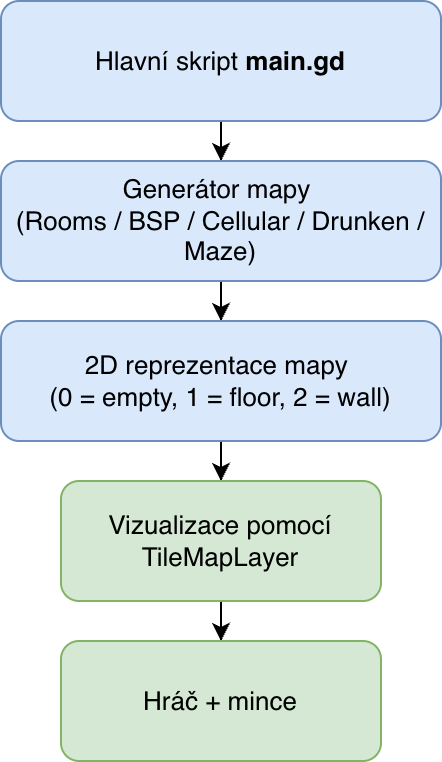
\includegraphics[width=0.4\textwidth]{images/generator_architecture.png}
\caption{Schéma architektury systému generování dungeonových map}
\label{fig:generator_architecture}
\end{figure}

\subsubsection{Vizualizace mapy a hráče}
Pro vizualizaci generovaných map byly v~aplikaci použity grafické prvky, takzvané assety. Tyto assety slouží především k~přehlednému zobrazení struktury generované mapy a~usnadňují orientaci uživatele. Vizualizace zahrnuje grafiku podlahy, stěn, postavy hráče a~sbíratelných objektů.

Zobrazení mapy je realizováno pomocí komponenty \texttt{TileMapLayer}. Po dokončení generování je datová reprezentace mapy předána funkci \\\texttt{\_draw\_map\_animated()}, která ji postupně převádí na odpovídající dlaždice, řádek po řádku s~krátkou prodlevou mezi jednotlivými řádky. Jednotlivé typy buněk jsou mapovány na konkrétní grafické prvky představující podlahu nebo stěnu. Tento způsob postupného vykreslování sice není nezbytný z~hlediska samotného generování, ale výsledná vizualizace působí přívětivěji.

Součástí prototypu je také jednoduchá reprezentace hráče, která slouží především k~ověření průchodnosti mapy. Umísťování hráče zajišťuje funkce \\ \texttt{\_place\_player\_on\_floor()}, která nejprve pomocí prohledávání do šířky (BFS) nalezne největší souvislou oblast průchozích dlaždic. V~této oblasti poté hledá pozici s~volným okolím $3 \times 3$ dlaždic, aby hráč nebyl ihned po vytvoření mapy zaseknut ve stěně. Pokud taková pozice neexistuje, je jako záložní řešení použita náhodná dlaždice z~největší oblasti. S~hráčem se lze jednoduše pohybovat pomocí kláves W, A, S, D. Po mapě se uživatel může pohybovat pravým tlačítkem myši, aniž by ovlivnil pozici hráče, pro návrat k~původní pozici slouží klávesa R.

Pro doplnění testovacího prostředí byly do mapy přidány sběratelné objekty ve formě mincí. Funkce \texttt{\_place\_coins\_on\_floor()} náhodně rozmístí 5 až 50 mincí na podlahové dlaždice v~největší souvislé oblasti mapy. Pokud hráč posbírá všechny mince, automaticky se vygeneruje nová mapa se stejnými parametry, jako v~případě předchozího generování. Tyto prvky neslouží jako hlavní součást PCG, jedná se pouze o~grafické doplnění.

V implementaci je využit volně dostupný balíček 2D Pixel Dungeon Asset Pack, jehož autorem je grafik vystupující pod jménem Pixel\_Poem. Tento balíček obsahuje základní sadu grafických prvků určených právě pro tvorbu dungeonových 2D her \cite{pixel_dungeon_asset}.

Použité assety mají podobu pixelové grafiky v~top-down perspektivě, tedy seshora dolů, a~svým návrhem přímo odpovídají práci s~dlaždicovou mapou, kterou engine využívá. Balíček je volně dostupný a~lze jej využít v~nekomerčních i~komerčních projektech.

Grafická vrstva -- hráč a~mince -- slouží pouze jako podpůrný nástroj pro vizualizaci výsledků generování.

\subsubsection{Ovládání generování a zobrazení statistik}

Součástí hry je jednoduché uživatelské rozhraní, které umožňuje výběr konkrétní generovací metody a~nastavení základních parametrů mapy -- šířky, výšky a~volitelného seedu. Je-li zaškrtnuto políčko seedu, je hodnota seedu předána generátoru a~výsledek generování je plně reprodukovatelný. Dále je možné nastavit počet opakování pro benchmarkový režim, přičemž výchozí hodnota je 200. Minimální hodnota seedu je 1.

Uživatelské rozhraní obsahuje dvě hlavní tlačítka, \textit{Generate} a~\textit{Benchmark}. Po stisknutí tlačítka \textit{Generate} skript, na základě uživatelské volby, vybere příslušný generátor pomocí konstrukce \texttt{match} a~zavolá jeho funkci \\ \texttt{generate(width, height, seed\_value)}, kde \texttt{seed\_value} je zadaná hodnota seedu, nebo 0, pokud seed není aktivní. Doba generování je dána pomocí funkce \\ \texttt{Time.get\_ticks\_usec()} a~měří výhradně volání generovací funkce, nikoli následné vykreslení mapy ani umísťování herních objektů, což zajistí to, že čas není ovlivněn samotným vykreslováním. Ihned po dokončení generování skript spočítá počet průchozích dlaždic a~procentuální pokrytí mapy a~zobrazí tyto údaje spolu s~časem generování v~uživatelském rozhraní. Výsledná mapa je poté vizualizována postupným vykreslováním jednotlivých řádků.

Tlačítko \textit{Benchmark} slouží k~automatizovanému testování všech implementovaných metod. Proces zajišťuje funkce \texttt{run\_benchmark()}, která postupně spustí všech pět algoritmů pro každou z~pěti definovaných velikostí map, přičemž každou konfiguraci opakuje konfigurovatelným počtem opakování (výchozí hodnota 200). Celkový počet generování v~rámci jednoho spuštění benchmarku je dán vzorcem $5 \times 5 \times \texttt{benchmark\_runs}$, kde první pětka odpovídá počtu algoritmů a~druhá počtu velikostí map. Průběh benchmarku je znázorněn pomocí ukazatele průběhu (progress bar), který průběžně zobrazuje procentuální dokončenost celkového počtu generování. Na rozdíl od běžného generování není při tomto režimu mapa vizualizována ani nejsou umísťovány herní objekty.

Výsledky jednotlivých běhů (algoritmus, rozměry, čas generování, pokrytí, počet podlahových dlaždic) jsou po každém běhu ukládány do souboru \\ \texttt{results.csv} pomocí funkce \texttt{\_log\_results()}, jejíž struktura je podrobněji popsána v~podkapitole věnované metodice měření.

\begin{figure}[H]
\centering
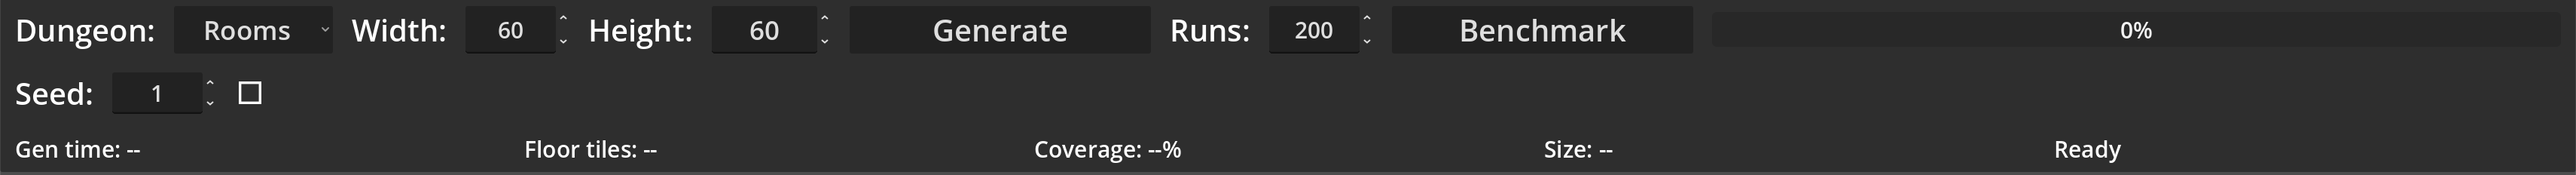
\includegraphics[width=0.8\textwidth]{images/ui_1.png}
\caption{Uživatelské rozhraní aplikace pro generování map}
\end{figure}


\subsection{Implementace generovacích metod}
Každý algoritmus z~kapitoly~\ref{sec:prehledMetod} je implementován jako samostatný skript v~adresáři \path{res://dungeons/algorithms}.

Všechny generátory sdílejí několik společných implementačních prvků. Každý skript rozšiřuje třídu \texttt{RefCounted}, nemá tedy vazbu na scénu, a~definuje trojici celočíselných konstant pro typy dlaždic: \texttt{TILE\_EMPTY = 0} (prázdný prostor), \texttt{TILE\_FLOOR = 1} (podlaha) a~\texttt{TILE\_WALL = 2} (stěna). Vstupním bodem je vždy statická funkce \texttt{generate(width, height, seed\_value)}, která vrací dvourozměrné pole představující výslednou mapu.

Na začátku funkce \texttt{generate()} každý generátor vytvoří lokální instanci \texttt{RandomNumberGenerator}. Pokud je předaný parametr \texttt{seed\_value} větší než 0, je seed nastaven voláním \texttt{rng.seed~=~seed\_value}, čímž je zajištěna plná reprodukovatelnost výsledků. V~opačném případě je zavolána metoda \texttt{rng.randomize()}, která zajistí unikátní průběh náhodných operací bez ovlivnění zbytku aplikace. Následně je inicializována prázdná mapu o~rozměrech \texttt{width} $\times$ \texttt{height}, kde jsou všechny buňky nastaveny na hodnotu \texttt{TILE\_EMPTY}. Výjimkou je generátor Buněčných automatů, který inicializaci mapy a~náhodnou počáteční výplň provádí v~jednom kroku. Podrobněji je tento postup popsán v~příslušné podkapitole.

Závěrečným krokem je doplnění stěn pomocí funkce \texttt{\_add\_walls()}, jejíž implementace je ve všech skriptech totožná. Funkce prochází celou mapu a~pro každou dlaždici podlahy kontroluje osm okolních buněk (Mooreovo sousedství). Pokud se v~sousedství nachází buňka \texttt{TILE\_EMPTY}, je změněna na \texttt{TILE\_WALL}. Tímto postupem vznikne souvislé ohraničení všech průchozích částí mapy bez nutnosti generovat stěny explicitně během samotného algoritmu. Kontrola hranic mapy zajišťuje, že se při zápisu stěn nepřistupuje mimo rozsah pole.

\subsubsection{Náhodné generování místností a~chodeb}

Implementace algoritmu se nachází v~souboru \texttt{rooms\_generator.gd}.

Počet generovaných místností je odvozen od celkové plochy mapy podle vzorce \\ \texttt{room\_count = max(5, width * height / AREA\_PER\_ROOM)}. \\ Hodnota konstanty \texttt{AREA\_PER\_ROOM = 360} vychází z~odhadu průměrné plochy, kterou jedna místnost včetně svého okolí v~mapě zabírá. Šířka i~výška místnosti jsou generovány náhodně v~rozmezí 6 až 16 dlaždic, průměrná velikost místnosti tedy činí přibližně $11 \times 11 = 121$ dlaždic. 

Kromě samotné plochy místnosti je však nutné počítat také s~prostorem, který zabírají chodby, stěny a~povinné jednopolíčkové mezery mezi místnostmi. Na základě empirického pozorování je tento faktor přibližně trojnásobkem plochy místnosti, tedy $121 \times 3 \approx 360$ dlaždic na jednu místnost. Na malých mapách je tak vygenerováno alespoň pět místností, zatímco na velkých mapách počet místností úměrně roste s~plochou. Maximální počet pokusů o~umístění místnosti je stanoven jako \texttt{room\_count * 10}, což zajišťuje dostatečný prostor pro opakované pokusy v~případě kolizí s~již umístěnými místnostmi, a~zároveň zabraňuje nekonečnému cyklování na mapách, kde se požadovaný počet místností nedaří umístit.

Každá nová místnost je reprezentována obdélníkem typu \texttt{Rect2} s~náhodně vygenerovanými rozměry. Pozice levého horního rohu místnosti je následně určena tak, aby místnost zůstala uvnitř hranic mapy a~zároveň nebyla umístěna přímo na jejím okraji.

Před přidáním nové místnosti do mapy je provedena kontrola překryvu se všemi dříve umístěnými místnostmi. Tato kontrola je realizována pomocí metody \texttt{grow(1).intersects(other)}, což znamená, že se testuje nejen skutečný průnik obdélníků, ale i~jejich rozšíření o~jednu dlaždici na každou stranu. V~praxi tak mezi dvěma místnostmi vždy zůstává alespoň jednopolíčková mezera. Pokud by se nová místnost překrývala s~některou z~již existujících, je zahozena a~algoritmus pokračuje dalším pokusem.

V~případě, že nová místnost překryv nevykazuje, je přidána do seznamu místností a~její vnitřní plocha je zapsána do mapy jako podlaha. To je realizováno dvojicí vnořených cyklů, které procházejí všechny buňky uvnitř obdélníku místnosti a~nastavují jejich hodnotu na \texttt{TILE\_FLOOR}. Tím dojde k~vyznačení průchozí oblasti odpovídající nové místnosti.

Každá nová místnost je následně propojena chodbou s~předchozí místností v~pořadí umístění. První místnost je z~tohoto propojování vyloučena, protože v~okamžiku jejího přidání ještě neexistuje žádná jiná místnost. Pro propojení se využívají středy obou místností získané pomocí metody \texttt{get\_center()}. Vlastní vytvoření chodby zajišťuje pomocná funkce \texttt{\_carve\_corridor()}, \\ která mezi dvěma zadanými body vyznačí chodbu tvaru písmene L. Algoritmus náhodně rozhoduje, zda bude chodba nejprve vedena ve vodorovném a~poté ve svislém směru, nebo opačně. Díky tomu výsledné mapy nepůsobí podobně.

Chodba není tvořena pouze jednou dlaždicí, ale má nastavitelnou šířku. V~implementaci je výchozí hodnota parametru \texttt{corridor\_width} nastavena na 2. Výsledná chodba je tedy široká 2 dlaždice a~při zápisu dlaždic chodby je současně kontrolováno, zda se zapisované souřadnice nacházejí uvnitř hranic mapy, a~to pomocí pomocné funkce \texttt{\_in\_bounds()}.

\begin{figure}[H]
\centering
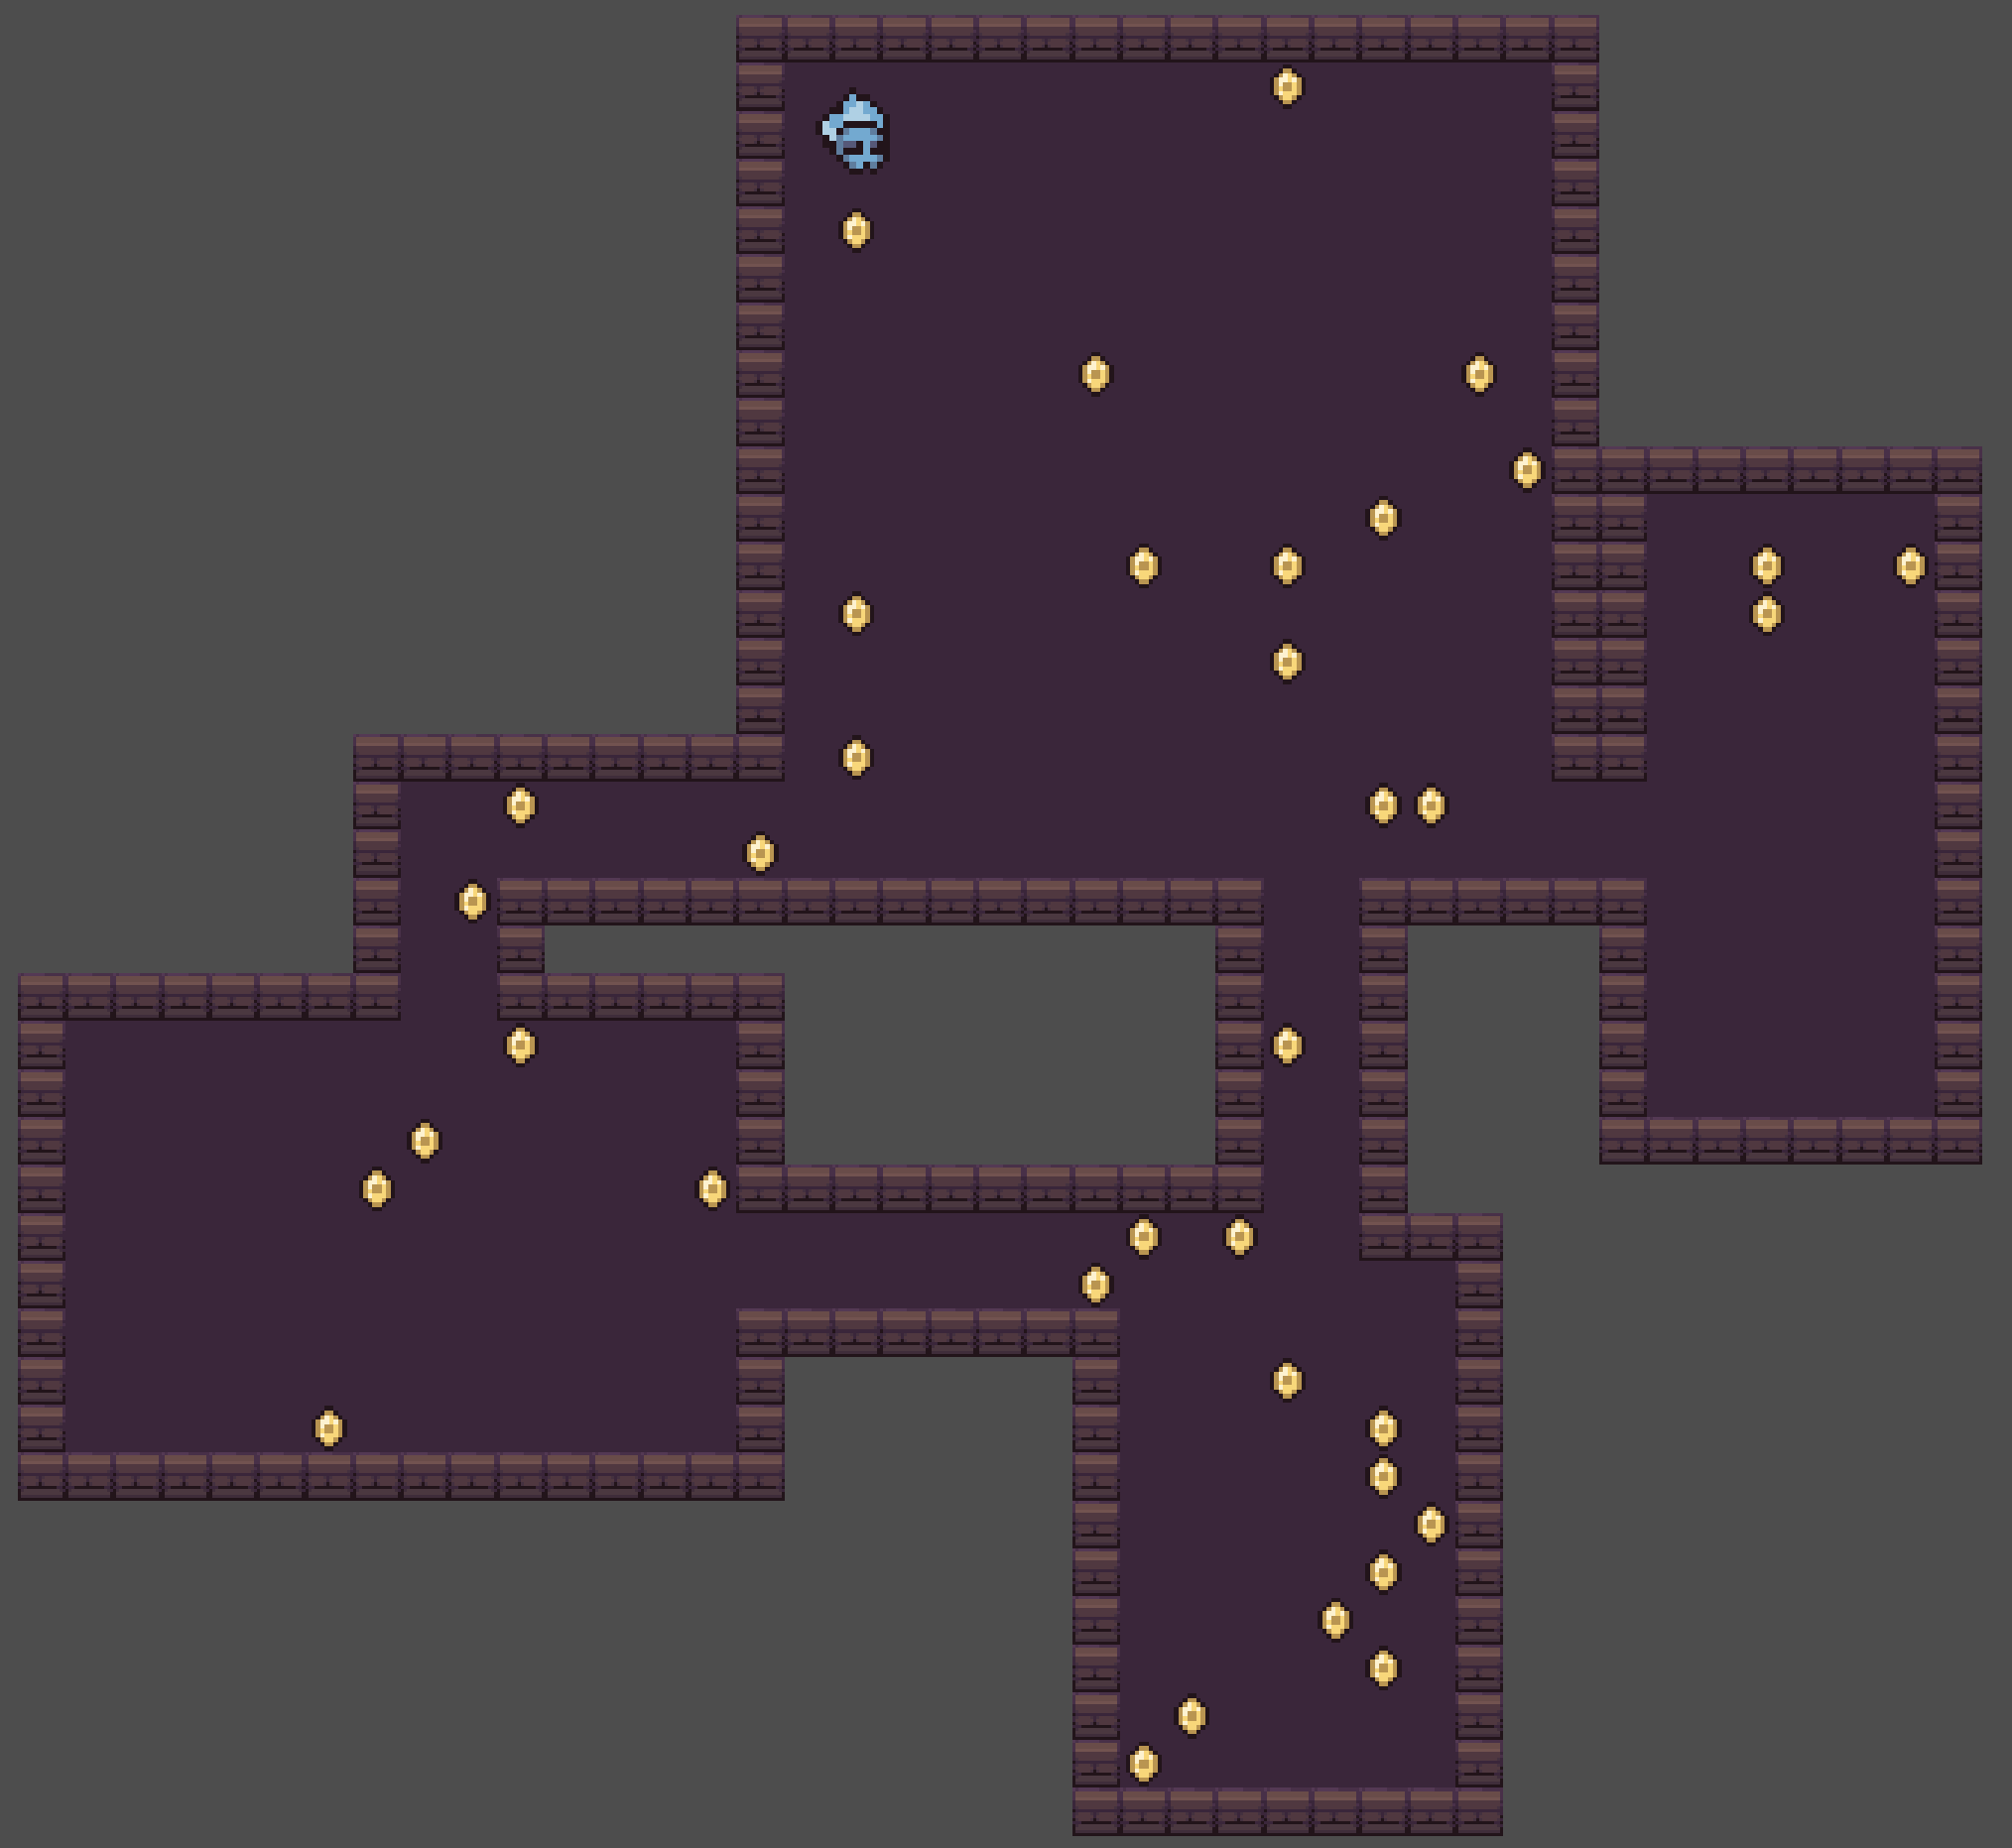
\includegraphics[width=0.7\textwidth]{images/rooms_45x45.png}
\caption{Ukázka mapy generované pomocí algoritmu náhodných místností a~chodeb (45$\times$45)}
\label{fig:rooms_45x45}
\end{figure}

\subsubsection{Binary Space Partitioning}

Implementace metody BSP se nachází v~souboru \texttt{bsp\_generator.gd}.

Stromová struktura mapy je reprezentována pomocnou třídou \texttt{Branch}. \\Každý uzel uchovává svou pozici (\texttt{Vector2i}), velikost (\texttt{Vector2i}) a~náhodné odsazení \texttt{padding} typu \texttt{Vector4i}, jehož složky udávají vzdálenost místnosti od okraje oblasti, náhodně 2 až 3 dlaždice na každé straně. Díky tomuto odsazení nevznikají místnosti těsně u~hranic oblastí a~mezi nimi zůstává dostatečný prostor.

Kořenový uzel pokrývá celou mapu zmenšenou o~jednu dlaždici na každé straně, tedy oblast od pozice $(1, 1)$ o~velikosti $(\texttt{width} - 2) \times (\texttt{height} - 2)$. Tím je na okraji mapy ponechán jednopolíčkový rámec.

Rekurzivní dělení prostoru provádí metoda \texttt{split(min\_size, rng)}. \\Směr řezu je určen deterministicky. Pokud je výška oblasti větší nebo rovna šířce (\texttt{size.y >= size.x}), dělí se horizontálně, jinak vertikálně. Dělení je ukončeno, pokud by výsledné podoblasti byly menší než \texttt{min\_size $\times$ 2}. Pozice řezu je volena náhodně v~rozmezí 35--65\,\% délky dělené části, takže vzniklé podoblasti nemusí být stejně velké.

Funkce \texttt{split()} je volána s~hodnotou konstanty \texttt{MIN\_SIZE = 13} a~rekurzivně dělí prostor tak dlouho, dokud to velikost oblasti umožňuje. Počet výsledných listových uzlů tedy není fixní, ale závisí na rozměrech mapy. Na větších mapách vzniká více oblastí a~tím i~více místností.
V~každém listu je vykreslena místnost odpovídající ploše uzlu zmenšené o~jeho odsazení \texttt{padding}.

Teprve po dokončení celého stromu jsou chodby získány metodou \\\texttt{get\_corridor\_pairs()}. Ta prochází strom rekurzivně a~pro každý vnitřní uzel vybere první listový uzel z~levého a~pravého podstromu a~uloží dvojici jejich středů. Středy místností jsou vypočítány metodou \texttt{get\_room\_center()}, která zohledňuje odsazení \texttt{padding}, takže výsledný bod leží vždy uvnitř skutečné průchozí plochy místnosti, nikoliv jen v~geometrickém středu celé podoblasti. Každá chodba má tvar písmene L, nejprve vede ve vodorovném, a~poté ve svislém směru. Chodba je široká 2 dlaždice.

\begin{figure}[H]
\centering
\includegraphics[width=0.7\textwidth]{images/bsp_45x45.png}
\caption{Ukázka mapy generované pomocí algoritmu BSP (45$\times$45)}
\label{fig:bsp_45x45}
\end{figure}

\subsubsection{Metoda Náhodné procházky}

Metoda Náhodné procházky se nachází v~souboru \\ \texttt{drunkards\_generator.gd}. Algoritmus začíná ve středu mapy na pozici \\ \texttt{width/2}, \texttt{height/2}. Kolem počáteční pozice je ihned vytvořena oblast podlahy o~velikosti $3 \times 3$ dlaždic pomocí funkce \texttt{\_carve\_3x3()}. Cílový počet průchozích dlaždic je stanoven na 50\,\% celkové plochy mapy podle vzorce~(\ref{eq:drunkards_target}), kde konstanta \textit{TARGET\_COVERAGE} je zmíněných 50.

\begin{equation}
\label{eq:drunkards_target}
\textit{cílový\_počet} = \frac{\textit{width} \times \textit{height} \times \textit{TARGET\_COVERAGE}}{100}
\end{equation}

Samotné generování probíhá v~cyklu, který pokračuje, dokud počet podlahových dlaždic nedosáhne cílového počtu. V~každém kroku je náhodně zvolen jeden ze čtyř směrů (nahoru, dolů, doleva, doprava) a~pozice generátoru se posune o~jednu dlaždici. Pozice je následně omezena funkcí \texttt{clamp()} tak, aby zůstávala alespoň 2 dlaždice od okraje mapy. Tato rezerva zajišťuje, že i~při vykreslování oblastí $3 \times 3$ nedojde k~překročení hranic pole.

Algoritmus rozlišuje dva typy vykreslování. Každých 15 až 25 kroků (interval je volen náhodně) je na aktuální pozici vytvořena oblast $3 \times 3$ dlaždic, která představuje malou místnost. V~ostatních krocích je vykreslena pouze oblast $2 \times 2$ dlaždic, což odpovídá chodbovému úseku. Obě varianty jsou realizovány jedinou pomocnou funkcí \texttt{\_carve\_area()}, které se předá požadovaná velikost oblasti (3 nebo 2). Funkce zapisuje podlahu pouze tam, kde dosud podlaha nebyla, a~vrací počet nově vytvořených dlaždic, aby mohl být průběžně aktualizován celkový počet.

Průchodnost celé mapy je zaručena tím, že veškerý průchozí prostor vzniká z~jedné souvislé procházky. Díky pevně stanovenému cílovému podílu podlahy je pokrytí mapy pro danou velikost relativně stabilní. Variabilita se projevuje především ve tvaru a~rozmístění vytvořených prostorů.

\begin{figure}[H]
\centering
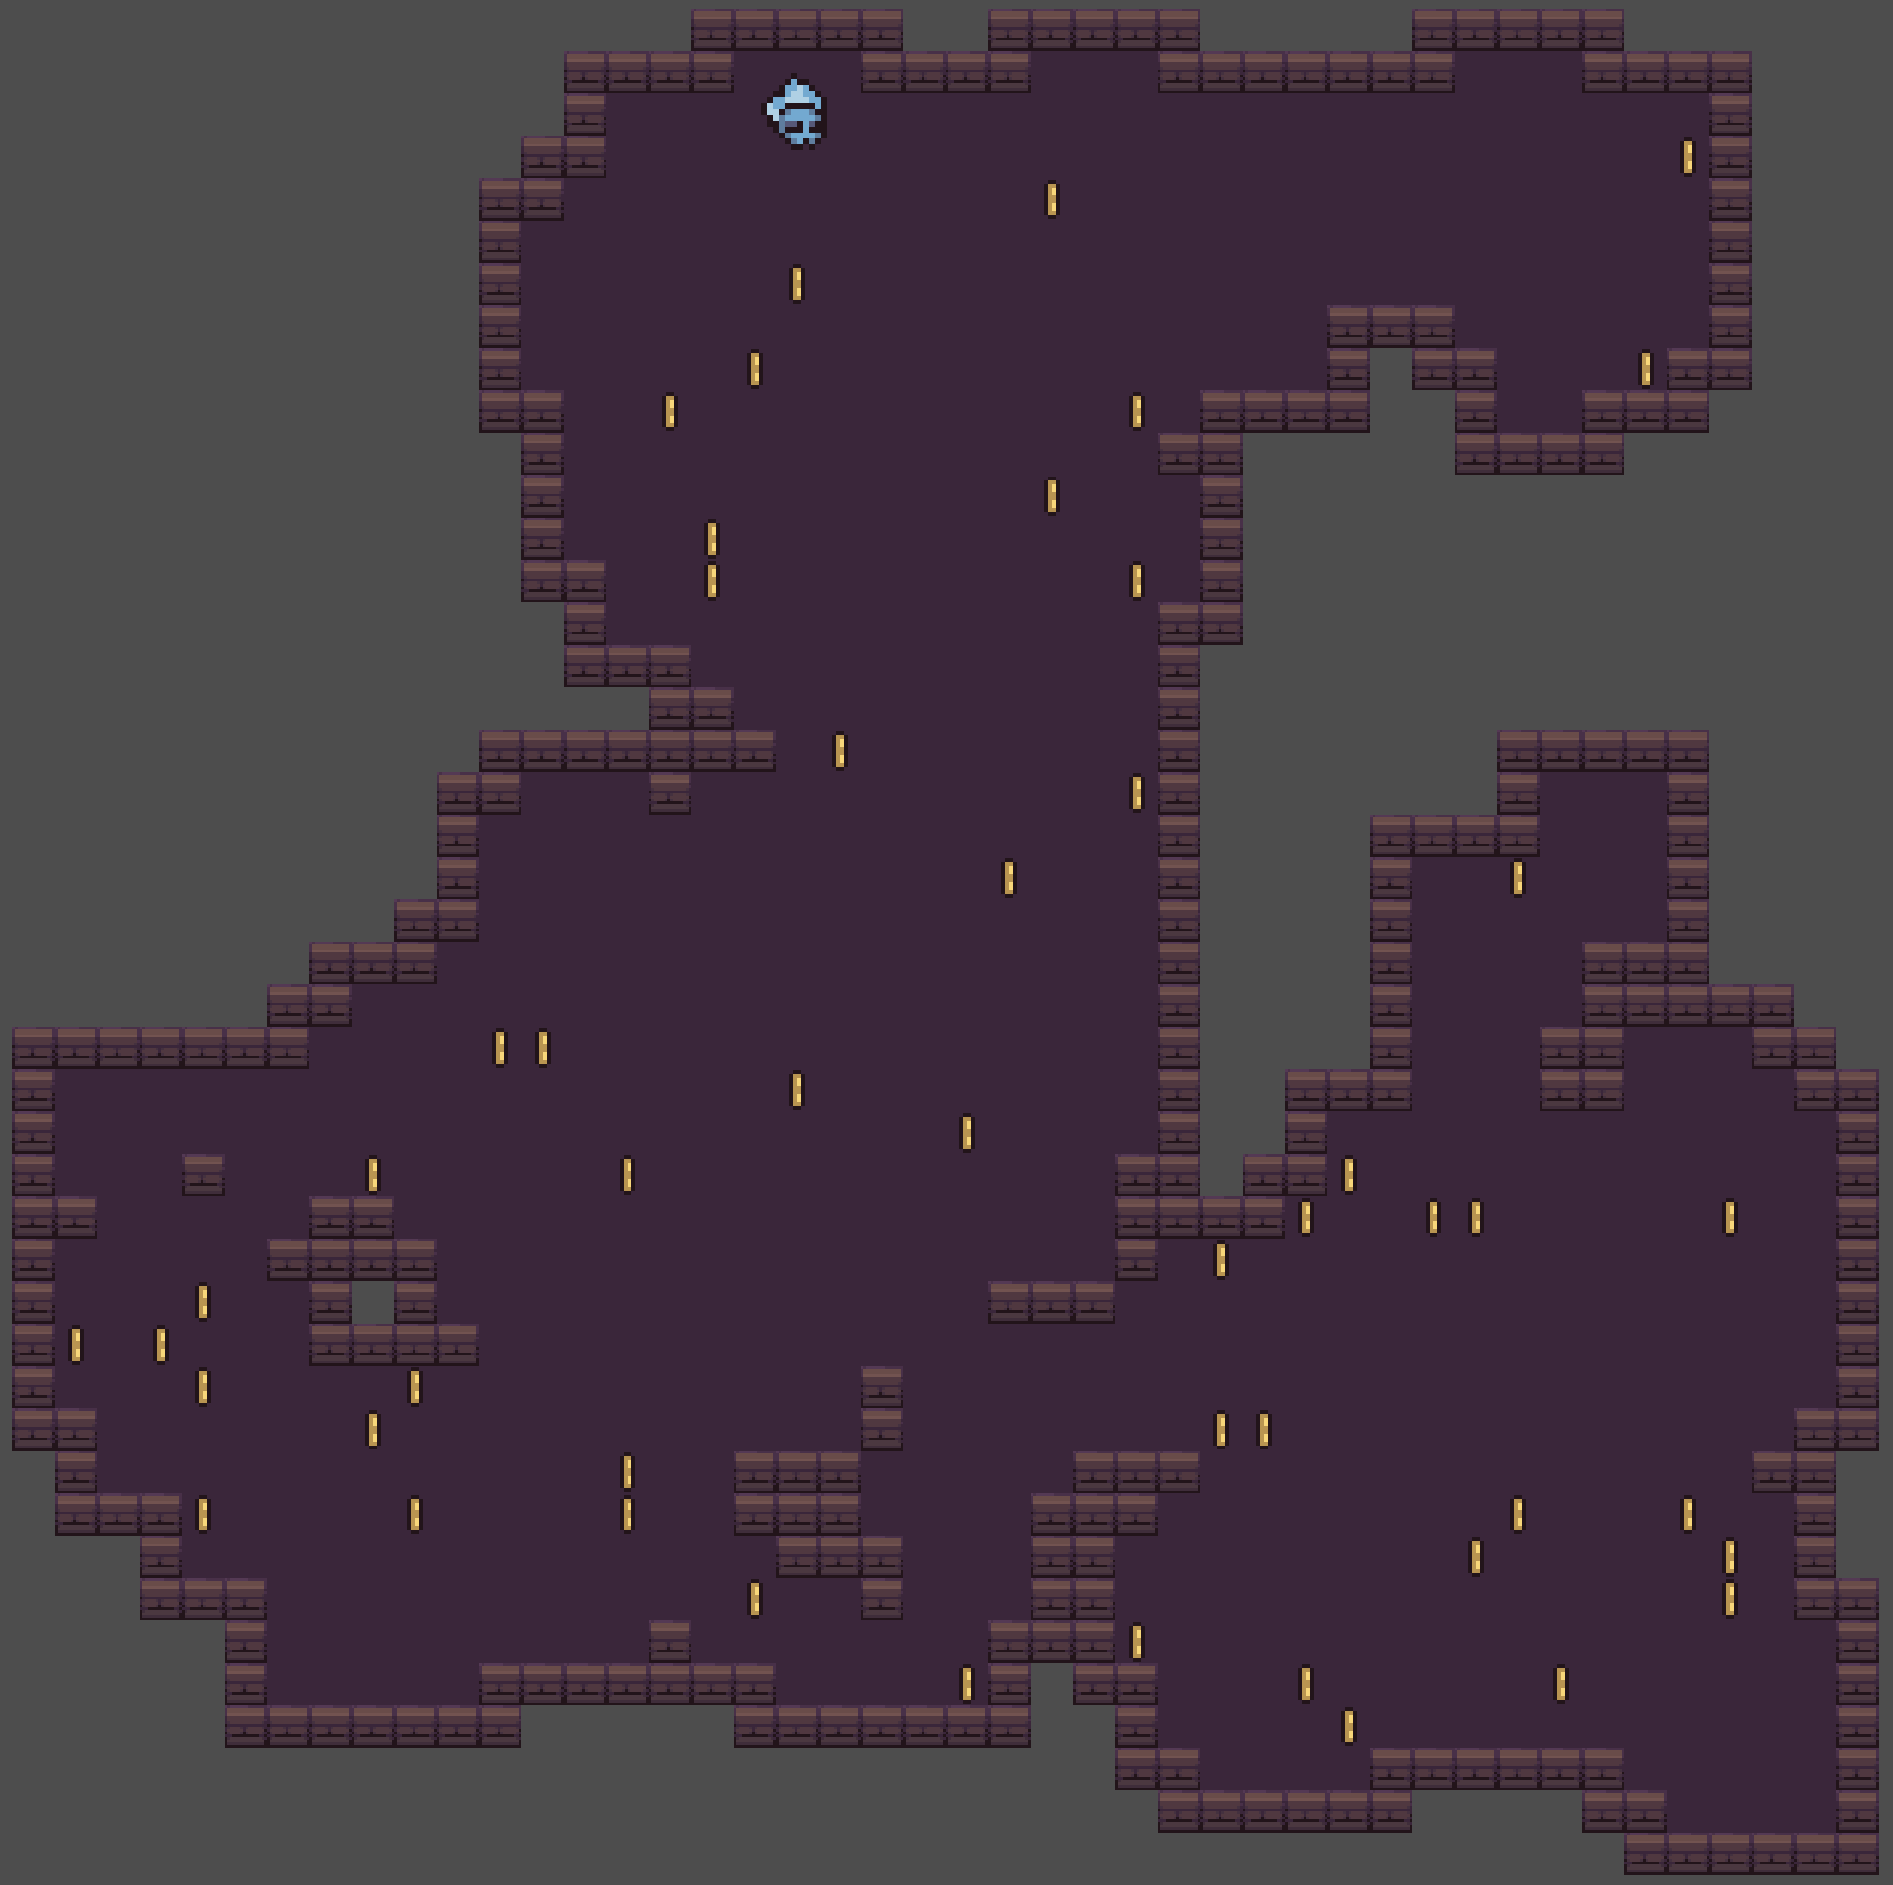
\includegraphics[width=0.7\textwidth]{images/drunkards_45x45.png}
\caption{Ukázka mapy generované pomocí algoritmu Náhodné procházky (45$\times$45)}
\label{fig:drunkards_45x45}
\end{figure}

\subsubsection{Buněčné automaty}

Implementace Buněčných automatů je v~souboru \texttt{cellular\_generator.gd}. 

V~první fázi je každá vnitřní buňka mapy náhodně nastavena na podlahu s~pravděpodobností \texttt{FILL\_PROBABILITY = 0.45}, tedy 45\,\%. Buňky na okraji mapy (první a~poslední řádek a~sloupec) zůstávají vždy prázdné, čímž vznikne pevný rámec, který zabraňuje rozšíření jeskynních prostor až k~hranicím pole.

Následuje celkem 5 simulačních kroků, které určuje konstanta \\ \texttt{SIMULATION\_STEPS}. V~každém kroku je vytvořena nová mapa, aby se průběžné změny nepromítaly do výpočtu sousedů v~témže kroku. Pro každou buňku funkce \texttt{\_count\_floor\_neighbours()} spočítá počet podlahových sousedů v~Mooreově okolí (osm přilehlých buněk). Pokud je tento počet alespoň 4, buňka se stane podlahou, v~opačném případě zůstane prázdná. Okrajové buňky ve všech krocích zůstávají prázdné.

Opakováním tohoto pravidla se náhodný šum postupně vyhladí do organických tvarů připomínajících jeskynní systémy. Volba počáteční pravděpodobnosti 45\,\% a~prahu 4 sousedů představuje kompromis mezi dostatečně otevřenými prostory a~přirozeně působícími stěnami. Při vyšší hodnotě by vznikaly příliš velké otevřené části, při nižší by byly oblasti méně průchozí, protože by velká část buněk tvořila stěny.

U map generovaných touto metodou se mohou vyskytovat izolované průchozí oblasti, protože algoritmus nezaručuje souvislost prostoru. Z~tohoto důvodu bylo při umisťování hráče nutné zohlednit průchozí plochu a~upřednostnit umístění do největší spojité oblasti mapy, což bylo nakonec zahrnuto ve všech metodách.

\begin{figure}[H]
\centering
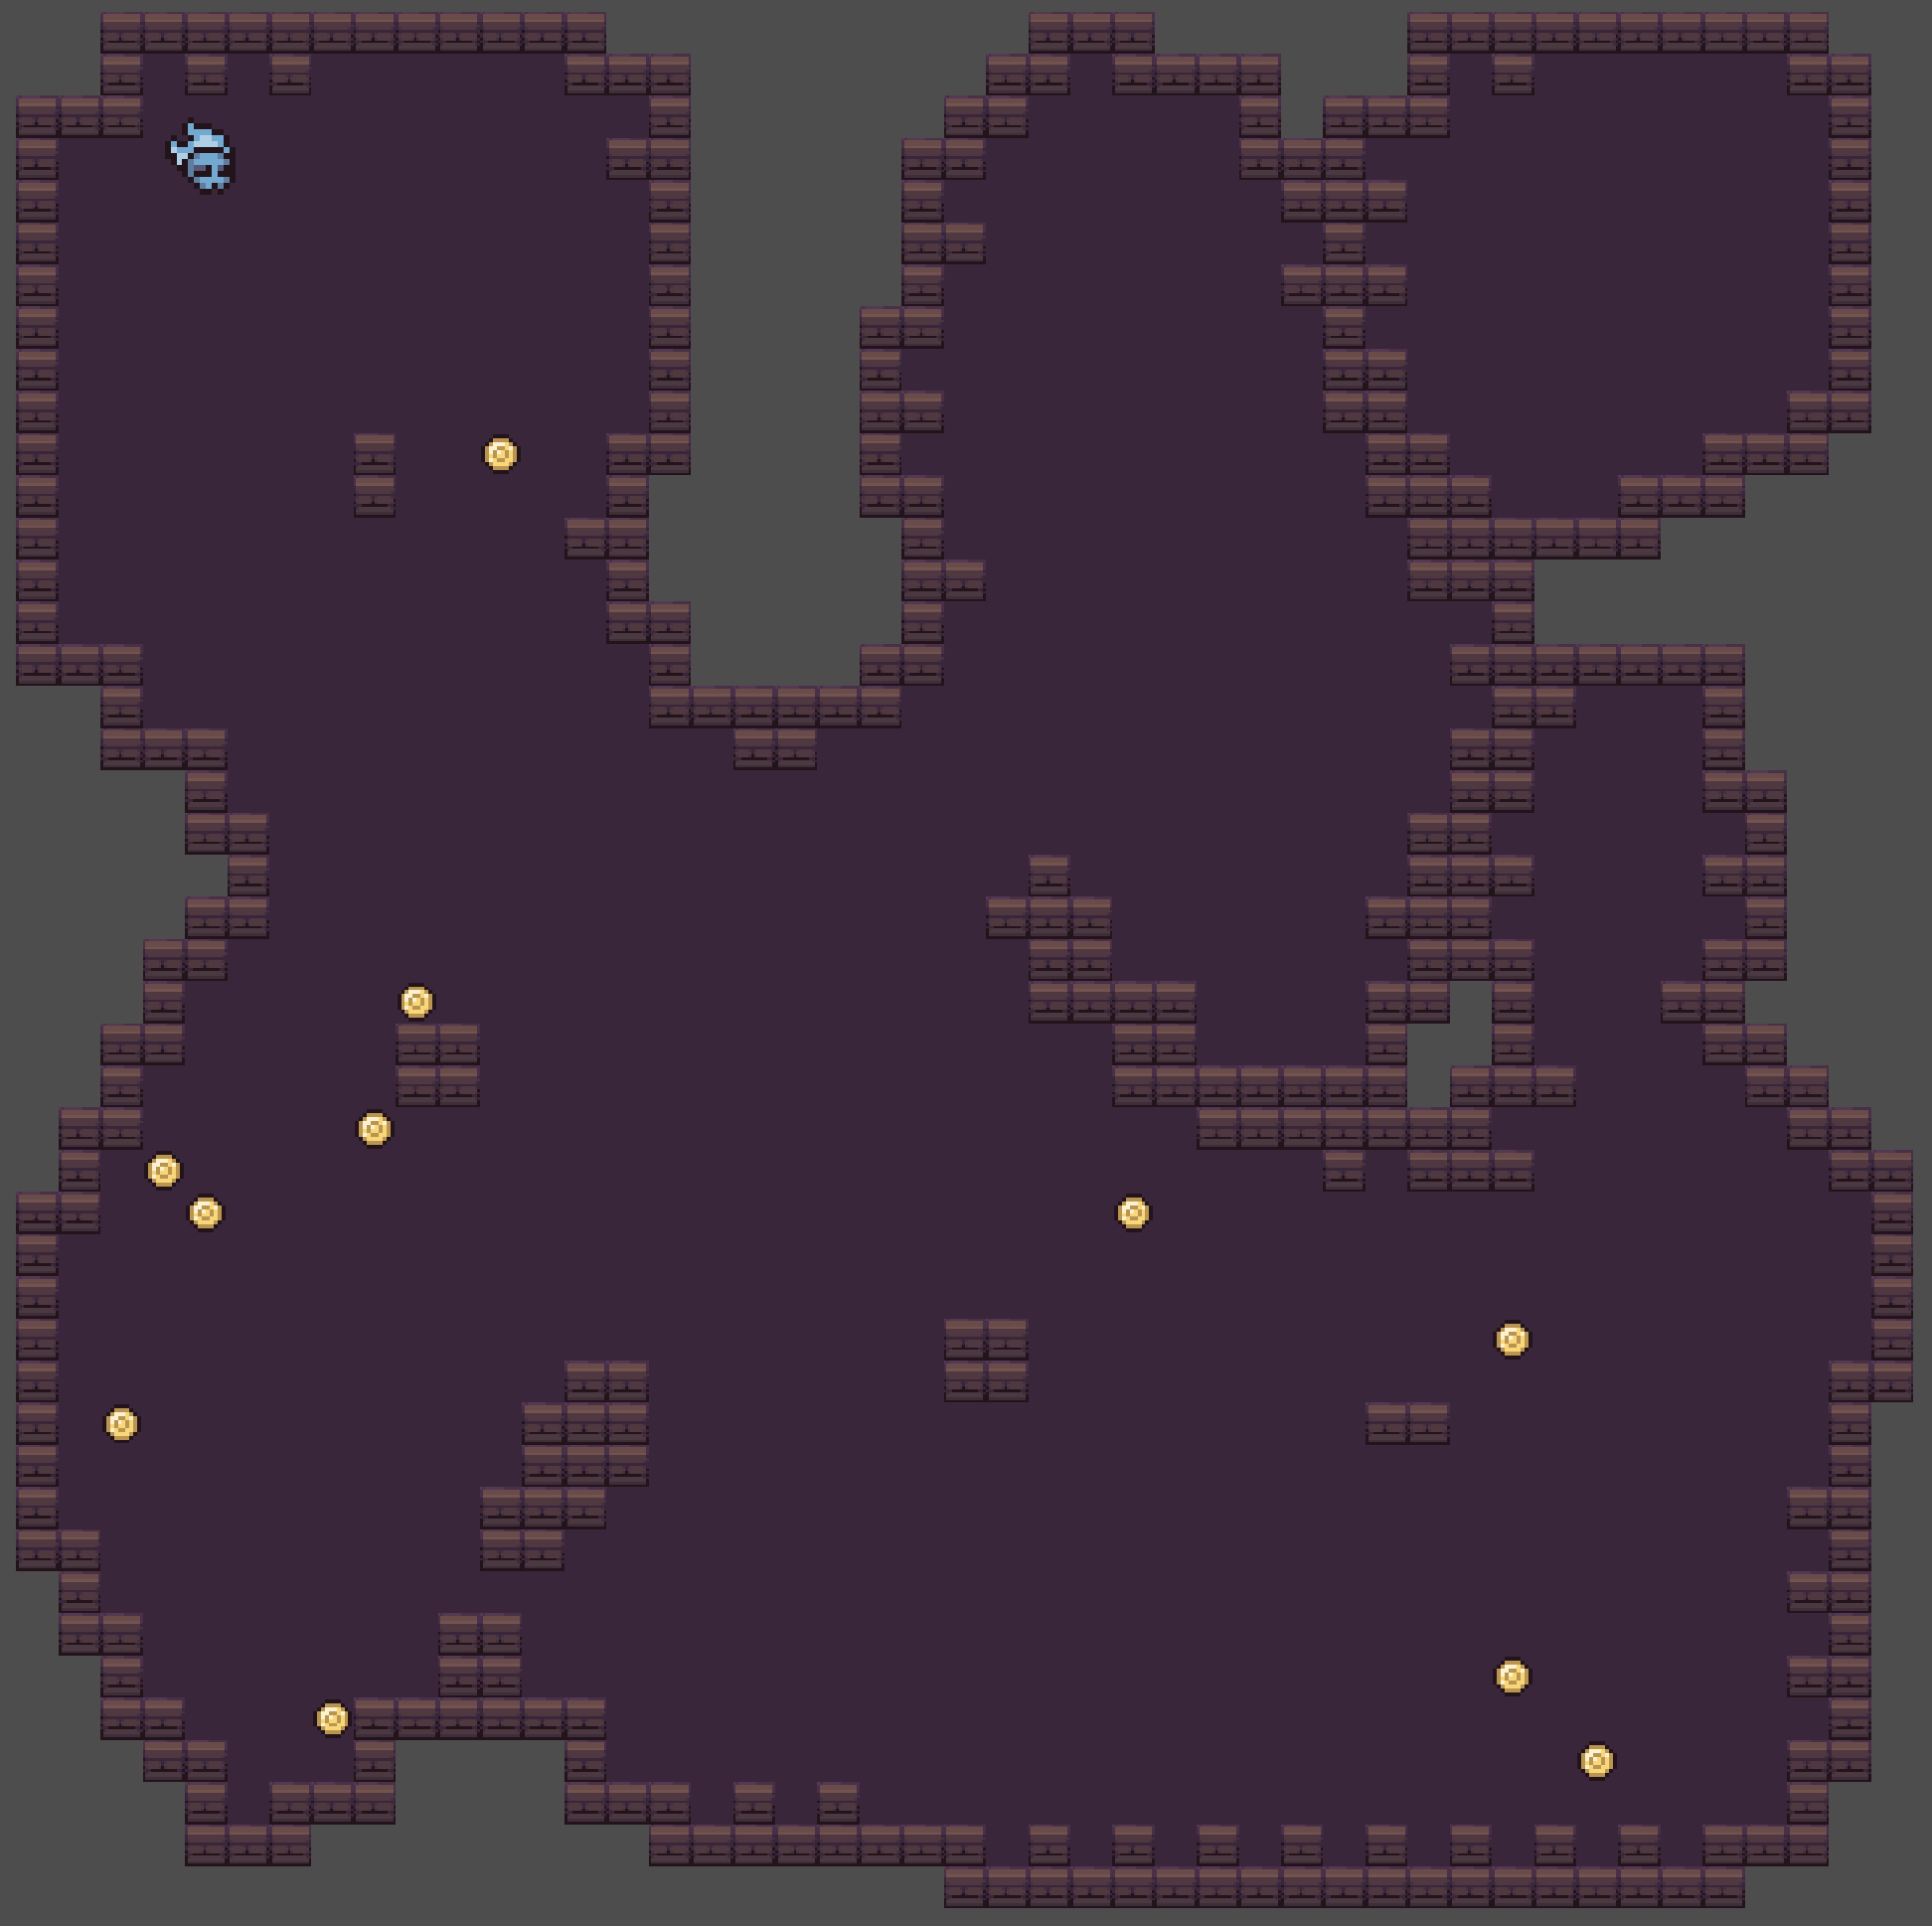
\includegraphics[width=0.7\textwidth]{images/cellular_45x45.png}
\caption{Ukázka mapy generované pomocí algoritmu Buněčných automatů (45$\times$45)}
\label{fig:cellular_45x45}
\end{figure}

\subsubsection{Metoda Bludiště}

Metoda Bludiště je implementována v~souboru \texttt{maze\_generator.gd}.

Implementace metody vychází z~algoritmu \textit{recursive backtracker} (prohledávání do hloubky se zásobníkem). Mapa je nejprve rozdělena na mřížku abstraktních buněk. Každá buňka zabírá $2 \times 2$ dlaždic podlahy a~mezi sousedními buňkami je jednodlaždicová mezera, takže na jednu buňku připadá úsek $3 \times 3$ dlaždic. Počet buněk závisí na rozměrech mapy, kde odečtení 2 zohledňuje jednodlaždicový okraj mapy na obou stranách:
\begin{equation}
    \texttt{cells\_w} = \max\!\Bigl(1,\, \Bigl\lfloor\frac{\texttt{width} - 2}{3}\Bigr\rfloor\Bigr), \qquad
    \texttt{cells\_h} = \max\!\Bigl(1,\, \Bigl\lfloor\frac{\texttt{height} - 2}{3}\Bigr\rfloor\Bigr).
\end{equation}

Stav každé buňky je zakódován jako bitová maska čtyř stěn (\texttt{N = 1}, \texttt{E = 2}, \texttt{S = 4}, \texttt{W = 8}), na začátku jsou všechny stěny přítomné. Algoritmus startuje v~buňce $(0, 0)$ a~v~každém kroku náhodně vybere nenavštíveného souseda. 
Ze společné stěny mezi aktuální buňkou a~vybraným sousedem je odstraněn příslušný bit na obou stranách, například při pohybu na sever se z~aktuální buňky odstraní bit \texttt{N} a~ze sousední buňky se odstraní bit \texttt{S}. Pokud aktuální buňka nemá žádného nenavštíveného souseda, algoritmus se vrací zpět po zásobníku. Průchod končí, jakmile jsou navštíveny všechny buňky.

Výsledkem je takzvané perfektní bludiště, ve kterém mezi libovolnými dvěma buňkami existuje právě jedna cesta. Po dokončení prohledávání je buněčná reprezentace převedena na dlaždicovou mapu. Každá buňka je vykreslena jako oblast $2 \times 2$ podlahových dlaždic na pozici $(1 + \texttt{cx} \cdot 3,\; 1 + \texttt{cy} \cdot 3)$. Tam, kde byla stěna odstraněna, je jednodlaždicová mezera mezi sousedními buňkami rovněž vyplněna podlahou o~šířce 2 dlaždic, čímž vznikne průchozí koridor.

\begin{figure}[H]
\centering
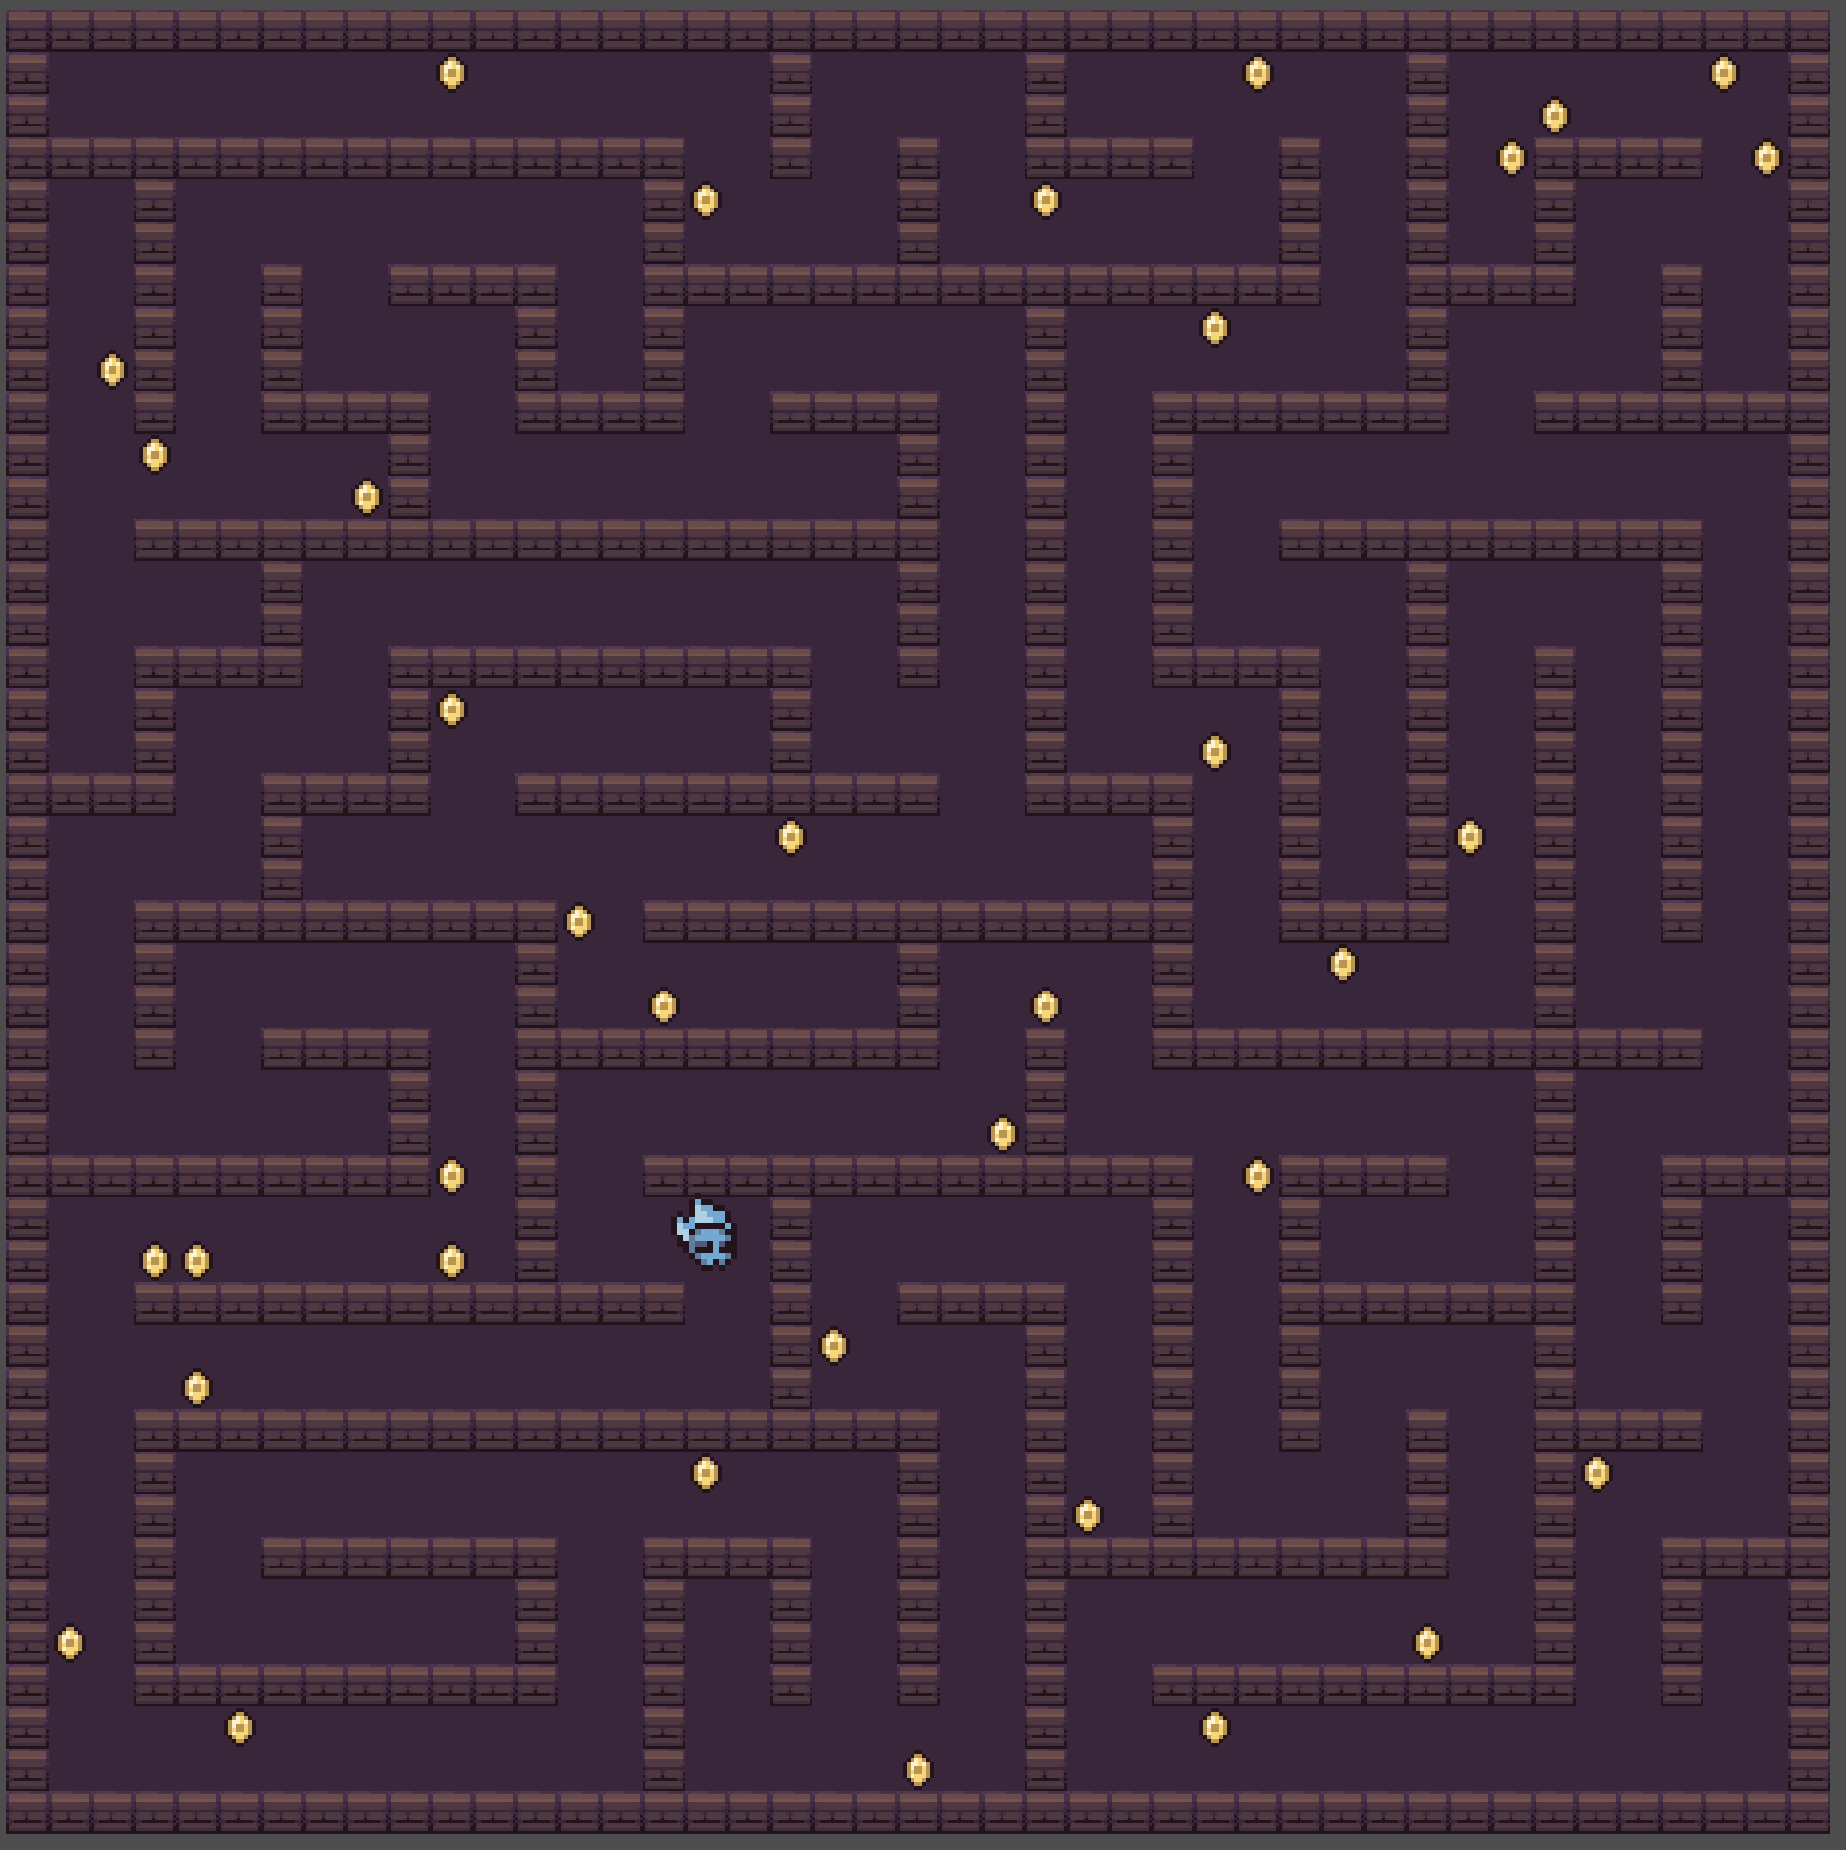
\includegraphics[width=0.7\textwidth]{images/maze_45x45.png}
\caption{Ukázka mapy generované pomocí algoritmu Bludiště (45$\times$45)}
\label{fig:maze_45x45}
\end{figure}


\subsection{Metodika měření a vyhodnocení}

Pro objektivní porovnání implementovaných algoritmů byl navržen automatizovaný benchmarkový režim, který je součástí aplikace. Jeho spuštění zajišťuje tlačítko \textit{Benchmark} v~uživatelském rozhraní. Po aktivaci jsou postupně spuštěny všechny implementované generovací metody pro pět předem definovaných velikostí map: 20$\times$50, 60$\times$60, 70$\times$30, 100$\times$100 a~150$\times$150 dlaždic. Tyto velikosti byly zvoleny tak, aby pokrývaly jak malé, tak velké rozměry map a~zároveň umožňovaly posoudit vliv tvaru mapy (čtverec versus obdélník) na chování algoritmů.

Pro každou kombinaci algoritmu a~velikosti mapy je generování provedeno opakovaně v~2000 bězích se seedem \texttt{05102024}. Celkem bylo pořízeno 50\,000 záznamů. Díky pevnému seedu jsou výsledky plně reprodukovatelné a~pokrytí mapy je pro každou kombinaci algoritmu, velikosti mapy a~seedu vždy totožné.

Pomocí funkce \texttt{Time.get\_ticks\_usec()} bylo zajištěno měření času s~mikrosekundovou přesností. Měřen je výhradně čas funkce \texttt{generate(width, height, seed\_value)} příslušného algoritmu. Vizualizace mapy, vykreslování dlaždic, umisťování hráče a~další operace nejsou součástí měřeného intervalu. Výsledný čas je převeden na milisekundy.

Pro každý běh jsou zaznamenány následující metriky:
\begin{itemize}
\item \textbf{čas generování} (\texttt{gen\_time\_ms}) -- doba trvání samotného algoritmu \\ v~milisekundách
\item \textbf{počet podlahových dlaždic} (\texttt{floor\_tiles}) -- celkový počet průchozích buněk ve výsledné mapě
\item \textbf{pokrytí} (\texttt{coverage}) -- podíl průchozích dlaždic z~celkového počtu buněk mapy, vyjádřený v~procentech:
\begin{equation}
    \texttt{coverage} = \frac{\text{floor\_tiles}}{\text{width} \times \text{height}} \times 100
\end{equation}
\end{itemize}

Naměřené hodnoty jednotlivých běhů jsou průběžně ukládány do souboru \\ \texttt{results.csv}. 
Každý záznam obsahuje název algoritmu, rozměry mapy, pořadí běhu, čas generování, pokrytí a~počet podlahových dlaždic.

Pro vyhodnocení naměřených dat byl vytvořen samostatný skript \\ \texttt{result\_analyser.py} v~jazyce Python s~využitím knihoven \texttt{pandas} \\ a~\texttt{matplotlib}. 
Skript načte soubor \texttt{results.csv} a~pro každou kombinaci algoritmu a~velikosti mapy vypočítá souhrnné statistiky -- průměr, směrodatnou odchylku, minimum a~maximum času generování i~pokrytí. Tyto statistiky jsou uloženy do souboru \texttt{results\_summary.csv}. Následně skript automaticky vygeneruje sadu grafů: sloupcové grafy průměrného času a~pokrytí pro jednotlivé algoritmy, škálovací křivky v~závislosti na velikosti mapy, boxploty rozložení hodnot a~bodový graf kompromisu mezi rychlostí a~pokrytím. Všechny grafické výstupy použité v~následující kapitole byly vygenerovány tímto skriptem.

\section{Výsledky}

Tato kapitola představuje výsledky experimentálního měření implementovaných generovacích metod. Nejprve jsou analyzovány vlastnosti jednotlivých algoritmů z~hlediska času generování a~pokrytí mapy průchozím prostorem. Následně jsou algoritmy vzájemně porovnány a~výsledky shrnuty v~souhrnné tabulce.

Všechny grafy v~této kapitole byly vygenerovány z~dat naměřených benchmarkovým režimem popsaným v~předchozí podkapitole. Nadpisy os a~legendy grafů jsou uvedeny v~anglickém jazyce. Názvy algoritmů v~grafech odpovídají anglickým označením \textit{Rooms} (Místnosti), \textit{BSP}, \textit{Drunkard's} (Náhodná procházka), \textit{Cellular} (Buněčné automaty) a~\textit{Maze} (Bludiště). V~popiscích obrázků je uveden český překlad nadpisu grafu.


\subsection{Výsledky jednotlivých algoritmů}

\subsubsection{Místnosti a chodby}

Algoritmus náhodných místností a~chodeb vykazuje nízké časy generování na menších mapách. Na mapě 20$\times$50 přibližně 1,1 ms. S~rostoucí velikostí mapy čas narůstá výrazněji. Na mapě 150$\times$150 dosahuje průměrný čas přibližně 27,2 ms.

Pokrytí mapy průchozím prostorem roste s~velikostí mapy. Na menších mapách (20$\times$50, 70$\times$30) se pohybuje v~rozmezí 31,1--42,9 \%, na mapě 100$\times$100 činí 43,8 \% a~na mapě 150$\times$150 dosahuje 54,1 \%. Tento rostoucí trend je dán tím, že počet místností se odvíjí od celkové plochy mapy. Na větších mapách tak vzniká úměrně více místností, které efektivněji vyplňují dostupný prostor.

Variabilita časů generování je malá a~odpovídá přirozeným výkyvům systému při opakovaném spouštění.

\begin{figure}[H]
\centering

\includegraphics[width=0.75\textwidth]{images/graphs/rooms_time_by_size.png}
\caption{Rooms -- průměrný čas generování podle velikosti mapy}
\label{fig:rooms_time}
\end{figure}

\begin{figure}[H]
\centering

\includegraphics[width=0.75\textwidth]{images/graphs/rooms_coverage_by_size.png}
\caption{Rooms -- průměrné pokrytí podle velikosti mapy}
\label{fig:rooms_coverage}
\end{figure}


\subsubsection{Binary Space Partitioning}

Algoritmus BSP vytváří mapy s~dobře definovanými místnostmi a~systematickým propojením. Čas generování roste s~velikostí map, od přibližně 0,82 ms na mapě 20$\times$50 po 20,3 ms na mapě 150$\times$150. Tento nárůst odpovídá rekurzivní povaze algoritmu, který musí rozdělit celý prostor mapy a~následně propojit vzniklé místnosti.

Pokrytí mapy u~BSP roste s~velikostí mapy. Na nejmenší mapě 20$\times$50 činí pokrytí přibližně 42,5 \%, na mapě 150$\times$150 dosahuje hodnot kolem 52,6 \%. Pokrytí je dáno principem adaptivního dělení prostoru podle minimální velikosti oblasti, které na větších mapách vytváří proporcionálně více menších místností.

Variabilita času mezi běhy je u~BSP nízká, směrodatné odchylky jsou malé, což odpovídá determinističtější povaze rekurzivního dělení prostoru.

\begin{figure}[H]
\centering

\includegraphics[width=0.75\textwidth]{images/graphs/bsp_time_by_size.png}
\caption{BSP -- průměrný čas generování podle velikosti mapy}
\label{fig:bsp_time}
\end{figure}

\begin{figure}[H]
\centering

\includegraphics[width=0.75\textwidth]{images/graphs/bsp_coverage_by_size.png}
\caption{BSP -- průměrné pokrytí podle velikosti mapy}
\label{fig:bsp_coverage}
\end{figure}


\subsubsection{Náhodná procházka}

Algoritmus Náhodné procházky se od ostatních metod odlišuje zejména pokrytím mapy. Výsledné pokrytí se ve všech testovaných konfiguracích pohybuje v~rozmezí 50,0--50,1 \%, což přímo odpovídá implementaci, ve které je cílový počet průchozích dlaždic stanoven pevně.

Čas generování vykazuje výraznější variabilitu mezi jednotlivými běhy. Na mapě 20$\times$50 se průměrný čas pohybuje kolem 2,5 ms. Na největší mapě 150$\times$150 dosahuje přibližně 55,6 ms. Variabilita časů odpovídá přirozeným výkyvům systému při opakovaném spouštění. Hodnota 50 \% je nastavitelný parametr a~změnou této konstanty lze dosáhnout libovolného cílového pokrytí.

\begin{figure}[H]
\centering

\includegraphics[width=0.75\textwidth]{images/graphs/drunkards_time_by_size.png}
\caption{Náhodná procházka -- průměrný čas generování podle velikosti mapy}
\label{fig:drunkards_time}
\end{figure}

\begin{figure}[H]
\centering

\includegraphics[width=0.75\textwidth]{images/graphs/drunkards_coverage_by_size.png}
\caption{Náhodná procházka -- průměrné pokrytí podle velikosti mapy}
\label{fig:drunkards_coverage}
\end{figure}


\subsubsection{Buněčné automaty}

Buněčné automaty jsou z~testovaných algoritmů jednoznačně nejpomalejší. Na nejmenší mapě 20$\times$50 trvá generování přibližně 7,3 ms, na mapě 100$\times$100 již 78,2 ms a~na největší mapě 150$\times$150 dosahuje průměrný čas přibližně 177,7 ms. Hlavní příčinou je algoritmická náročnost. Algoritmus provádí 5 úplných průchodů přes všechny buňky mapy, přičemž pro každou buňku vyhodnocuje 8 okolních sousedů. To představuje řádově více operací než u~ostatních algoritmů. Interpretovaný jazyk GDScript může tento efekt dále zhoršovat v~porovnání s~kompilovanými jazyky, nicméně primární příčinou vysokého času zůstává samotná struktura algoritmu.

Pokrytí mapy u~Buněčných automatů dosahuje vysokých hodnot a~s~rostoucí velikostí mapy mírně roste. Od přibližně 59,4 \% na mapě 20$\times$50 po 72,3 \% na mapě 150$\times$150.

Čas generování je mezi běhy prakticky konstantní a~směrodatné odchylky jsou velmi malé. Celkový počet operací tak závisí primárně na velikosti mapy.

\begin{figure}[H]
\centering

\includegraphics[width=0.75\textwidth]{images/graphs/cellular_time_by_size.png}
\caption{Cellular automata -- průměrný čas generování podle velikosti mapy}
\label{fig:cellular_time}
\end{figure}

\begin{figure}[H]
\centering

\includegraphics[width=0.75\textwidth]{images/graphs/cellular_coverage_by_size.png}
\caption{Cellular automata -- průměrné pokrytí podle velikosti mapy}
\label{fig:cellular_coverage}
\end{figure}


\subsubsection{Bludiště}

Algoritmus generování Bludiště se vyznačuje zcela deterministickým pokrytím mapy. Hodnota pokrytí je pro danou velikost mapy vždy shodná bez ohledu na konkrétní běh. Na mapě 20$\times$50 činí pokrytí 57,4 \%, na mapě 150$\times$150 pak 64,0 \%. Nulová variabilita pokrytí vyplývá z~principu algoritmu recursive backtracker, který vždy navštíví všechny buňky mřížky a~výsledný poměr průchozích dlaždic je dán pouze rozměry mapy a~velikostí buněk.

Čas generování je u~tohoto algoritmu srovnatelný s~BSP. Na nejmenší mapě činí přibližně 1,18 ms, na největší pak 23,6 ms. Variabilita času mezi běhy je velmi nízká, protože algoritmus vždy provede stejný počet kroků.

\begin{figure}[H]
\centering

\includegraphics[width=0.75\textwidth]{images/graphs/maze_time_by_size.png}
\caption{Maze -- průměrný čas generování podle velikosti mapy}
\label{fig:maze_time}
\end{figure}

\begin{figure}[H]
\centering
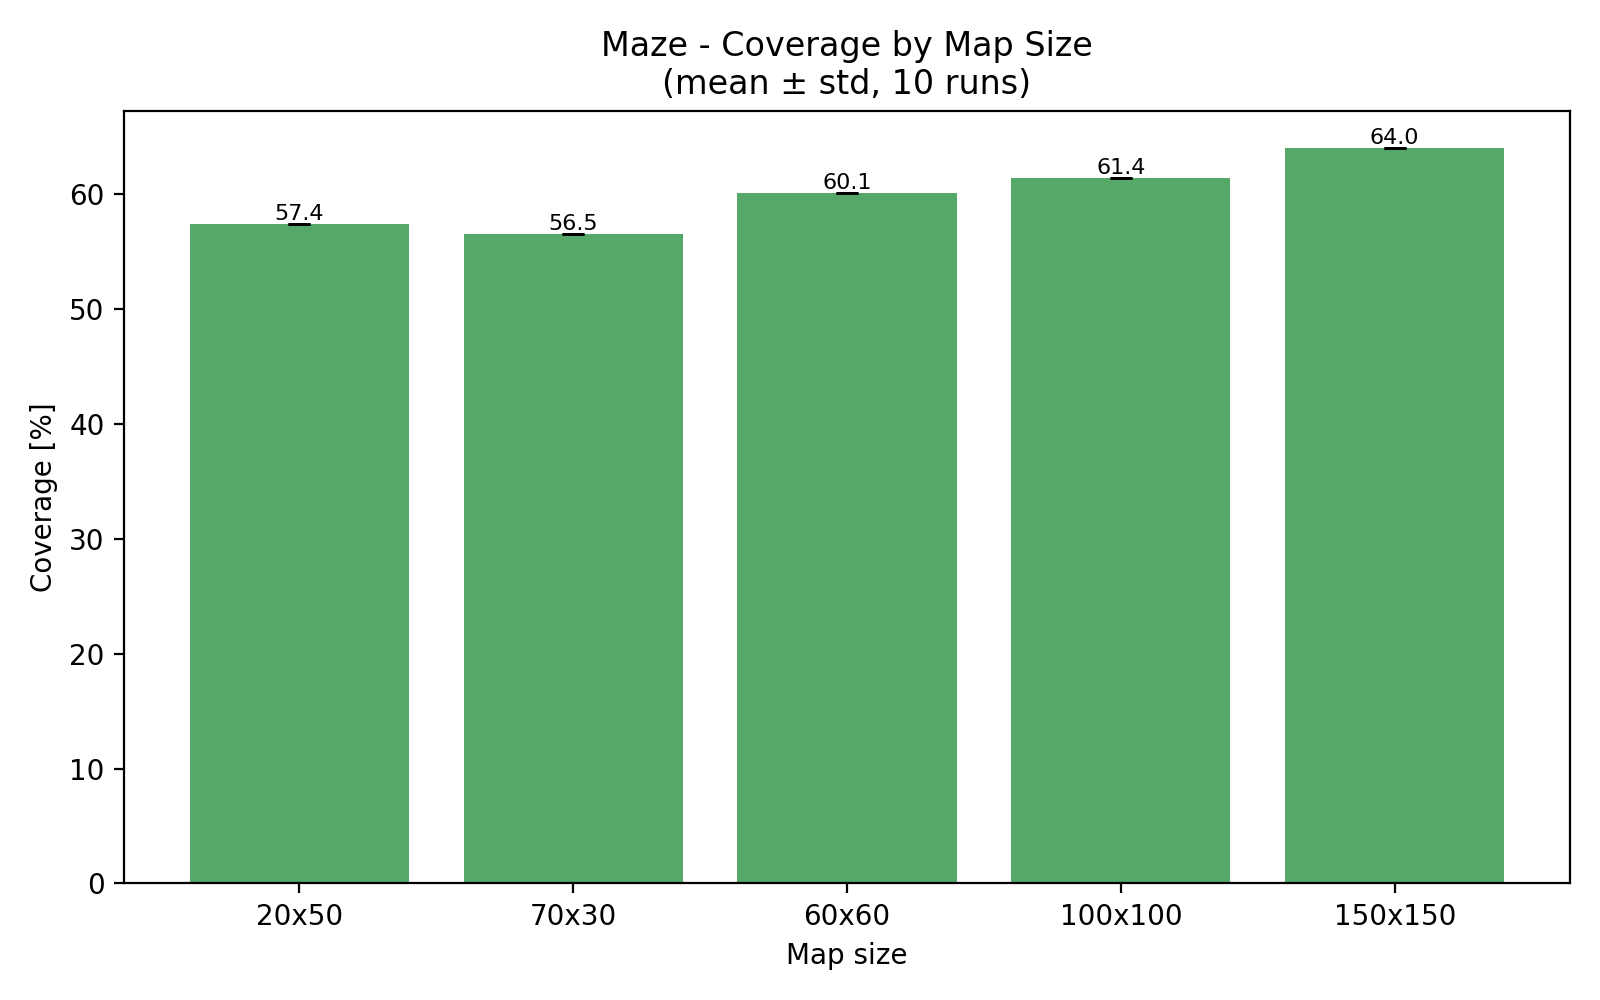
\includegraphics[width=0.75\textwidth]{images/graphs/maze_coverage_by_size.png}
\caption{Maze -- průměrné pokrytí podle velikosti mapy}
\label{fig:maze_coverage}
\end{figure}


\subsection{Srovnání algoritmů}

Tato podkapitola porovnává všechny implementované metody z~hlediska času generování, pokrytí mapy a~jejich vzájemného vztahu. Pokud není uvedeno jinak, zobrazené hodnoty představují průměry přes všechny testované velikosti map (2000 měření na každou kombinaci algoritmu a~velikosti, celkem 10\,000 měření na algoritmus). Konkrétní hodnoty pro jednotlivé velikosti jsou shrnuty v~tabulce \ref{tab:results_summary}.

\subsubsection{Průměrný čas generování}

Graf \ref{fig:comp_avg_time} zobrazuje průměrný čas generování algoritmů přes všechny testované velikosti map. 
Mezi algoritmy jsou patrné výrazné rozdíly. Nejrychlejšími metodami jsou BSP s průměrem 8,5 ms a~Bludiště s~průměrem 9,2 ms. Místnosti dosahují průměru 10,1 ms. Náhodná procházka je výrazně pomalejší s~celkovým průměrem 19,8 ms. Buněčné automaty jsou řádově nejpomalejší s~průměrem 61,3 ms, tedy přibližně sedmkrát více než u~BSP. 

\begin{figure}[H]
\centering

\includegraphics[width=0.75\textwidth]{images/graphs/comparison_avg_time.png}
\caption{Srovnání průměrného času generování všech algoritmů}
\label{fig:comp_avg_time}
\end{figure}

Na největší testované mapě 150$\times$150 jsou absolutní rozdíly ještě výraznější, BSP dosahuje 20,3 ms, Bludiště 23,6 ms, Místnosti 27,2 ms, Náhodná procházka 55,6 ms, zatímco Buněčné automaty přibližně 177,7 ms, jak lze vidět na grafu \ref{fig:comp_avg_time_150x150}.

\begin{figure}[H]
\centering

\includegraphics[width=0.75\textwidth]{images/graphs/comparison_time_150x150.png}
\caption{Srovnání průměrného času generování na mapě 150$\times$150}
\label{fig:comp_avg_time_150x150}
\end{figure}


\subsubsection{Průměrné pokrytí}

Graf \ref{fig:comp_avg_coverage} zobrazuje průměrné pokrytí mapy průchozím prostorem přes všechny testované velikosti. Nejvyššího celkového pokrytí dosahují Buněčné automaty (66,5 \%), následované algoritmem Bludiště se stabilním pokrytím 59,9 \%. BSP dosahuje celkového průměru 48,5 \%, Náhodná procházka má konstrukčně dané pokrytí 50,0 \%, které se s~velikostí mapy nemění. Místnosti a~chodby dosahují nejnižšího celkového průměru, a~to 40,9 \%, avšak pokrytí výrazně roste s~velikostí mapy (viz graf \ref{fig:comp_coverage_scaling}).

\begin{figure}[H]
\centering

\includegraphics[width=0.75\textwidth]{images/graphs/comparison_avg_coverage.png}
\caption{Srovnání průměrného pokrytí všech algoritmů}
\label{fig:comp_avg_coverage}
\end{figure}


\subsubsection{Škálování s velikostí mapy}

Graf \ref{fig:comp_time_scaling} znázorňuje, jak se čas generování mění s~rostoucím počtem buněk mapy. BSP a~Bludiště vykazují přibližně lineární nárůst času. Algoritmus Místností roste rovněž přibližně lineárně, avšak s~vyšší konstantou, protože na velkých mapách generuje výrazně více místností. Náhodná procházka roste rychleji, a~to kvůli opakovanému navracení do již odkrytých oblastí. Buněčné automaty vykazují nejstrmější nárůst.

\begin{figure}[H]
\centering

\includegraphics[width=0.85\textwidth]{images/graphs/comparison_time_scaling.png}
\caption{Škálování času generování s~počtem buněk mapy}
\label{fig:comp_time_scaling}
\end{figure}

Naměřené výsledky jsou v~souladu s~teoretickou časovou složitostí algoritmů. Všechny implementované metody dosahují lineární složitosti $O(n)$, kde $n = w \cdot h$ označuje celkový počet buněk mapy. Rozdíly v~rychlosti jsou způsobeny konstantními koeficienty. Buněčné automaty provádějí pro každou buňku $s = 5$ průchodů s~vyhodnocením 8~sousedů, tedy přibližně $40 \cdot n$ operací, což odpovídá přibližně osminásobnému rozdílu oproti algoritmům BSP a~Bludiště. Algoritmus Místností provádí kontrolu překryvů v~čase $O(r^2)$, kde $r = O(n/360)$, avšak tento výpočet je v~praxi zanedbatelný a~dominuje lineární průchod mapou při přidávání stěn. Stochastická povaha Náhodné procházky způsobuje opakované navštěvování odkrytých oblastí a~výraznou variabilitu doby generování, i~přes lineární průměrnou složitost.

Graf \ref{fig:comp_coverage_scaling} ukazuje vývoj pokrytí v~závislosti na velikosti mapy. BSP, Buněčné automaty a~Místnosti vykazují rostoucí tendenci, s~větší mapou roste i~podíl průchozího prostoru, což je očekávané. U~Místností je tento nárůst dán škálováním počtu místností s~plochou mapy. Bludiště má mírně rostoucí, ale velmi stabilní pokrytí. Náhodná procházka zůstává konstantní na hodnotě 50 \%.

Výjimku tvoří mapa 70$\times$30, u~které pokrytí algoritmů Místností, BSP a~Bludiště klesá pod hodnoty dosažené na mapě 20$\times$50, přestože celkový počet buněk je větší (2\,100 vs. 1\,000). Příčinou je především tvar mapy. Nízký obdélník omezuje rozmístění místností i~dělení prostoru. U~Místností se do výšky 30 dlaždic (28, pokud zahrneme okraje) nevejde plný počet místností minimální velikosti a~chodby zabírají větší podíl plochy. U~BSP a~Bludiště úzký tvar zmenšuje použitelné oblasti při dělení mřížky, čímž roste podíl stěn a~okrajů vůči prostoru, který je průchozí.

\begin{figure}[H]
\centering

\includegraphics[width=0.85\textwidth]{images/graphs/comparison_coverage_scaling.png}
\caption{Škálování pokrytí s~počtem buněk mapy}
\label{fig:comp_coverage_scaling}
\end{figure}


\subsubsection{Kompromis mezi rychlostí a pokrytím}

Graf \ref{fig:comp_tradeoff} vizualizuje vztah mezi průměrným časem generování a~průměrným pokrytím pro jednotlivé algoritmy (oba průměry přes všechny testované velikosti map). Ideální algoritmus by se nacházel v~levé horní části grafu, tedy s~nízkým časem a~vysokým pokrytím.

BSP a~Bludiště se nacházejí v~oblasti nízkého času a~středně vysokého pokrytí, přičemž Bludiště dosahuje vyššího pokrytí (59,9 \%) než BSP (48,5 \%). Místnosti nabízí srovnatelný čas s~nižším celkovým pokrytím. Buněčné automaty dosahují nejvyššího pokrytí ze všech metod, avšak za cenu výrazně vyššího výpočetního času. Náhodná procházka představuje předvídatelné pokrytí 50,0 \%, avšak s~vyšším časem generování než BSP, Bludiště a~Místnosti.

\begin{figure}[H]
\centering

\includegraphics[width=0.75\textwidth]{images/graphs/comparison_tradeoff.png}
\caption{Kompromis mezi rychlostí a~pokrytím}
\label{fig:comp_tradeoff}
\end{figure}


\subsubsection{Rozptyl výsledků na velké mapě}

Pro detailnější pohled na variabilitu výsledků jsou uvedeny boxploty času generování a~pokrytí na největší testované mapě 150$\times$150. 

Na obrázku \ref{fig:size150_time_box} je patrné, že BSP vykazuje nejmenší relativní rozptyl času, zatímco Náhodná procházka má nejvyšší variabilitu. 

\begin{figure}[H]
\centering

\includegraphics[width=0.75\textwidth]{images/graphs/size_150x150_time_boxplot.png}
\caption{Rozptyl času generování na mapě 150$\times$150}
\label{fig:size150_time_box}
\end{figure}

Obrázek \ref{fig:size150_cov_box} ukazuje, že při použití pevného seedu je pokrytí pro všechny algoritmy zcela deterministické a~variabilita pokrytí je nulová napříč všemi metodami.

\begin{figure}[H]
\centering

\includegraphics[width=0.75\textwidth]{images/graphs/size_150x150_coverage_boxplot.png}
\caption{Rozptyl pokrytí na mapě 150$\times$150}
\label{fig:size150_cov_box}
\end{figure}


\subsection{Souhrnná tabulka výsledků}

Tabulka \ref{tab:results_summary} shrnuje průměrné hodnoty času generování a~pokrytí mapy pro všechny testované kombinace algoritmů a~velikostí map.

\begin{table}[H]
\centering
\small
\begin{tabular}{|l|r|r|r|r|r|}
\hline
\textbf{Algoritmus} & \textbf{20$\times$50} & \textbf{60$\times$60} & \textbf{70$\times$30} & \textbf{100$\times$100} & \textbf{150$\times$150} \\
\hline
\multicolumn{6}{|c|}{\textit{Průměrný čas generování [ms]}} \\
\hline
Rooms    & 1,15  & 5,75  & 4,83  & 11,42  & 27,24  \\
BSP      & 0,82  & 6,21  & 4,31  & 10,67  & 20,30  \\
Drunkard's  & 2,50  & 9,68  & 8,81  & 22,44  & 55,57  \\
Cellular & 7,32  & 27,64 & 15,61 & 78,21  & 177,65 \\
Maze     & 1,18  & 4,20  & 5,62  & 11,40  & 23,63  \\
\hline
\multicolumn{6}{|c|}{\textit{Průměrné pokrytí [\%]}} \\
\hline
Rooms    & 42,90 & 32,53 & 31,10 & 43,81 & 54,09 \\
BSP      & 42,50 & 50,92 & 43,29 & 53,42 & 52,56 \\
Drunkard's  & 50,00 & 50,03 & 50,05 & 50,00 & 50,00 \\
Cellular & 59,40 & 65,94 & 63,95 & 70,91 & 72,26 \\
Maze     & 57,40 & 60,11 & 56,48 & 61,42 & 64,02 \\
\hline
\end{tabular}
\caption{Průměrný čas generování a~pokrytí}
\label{tab:results_summary}
\end{table}


\subsection{Shrnutí výsledků}

Na základě provedených měření lze algoritmy rozdělit do tří skupin podle výpočetní náročnosti. Do první skupiny patří BSP, Bludiště a~Místnosti, jejichž časy generování na mapě 150$\times$150 nepřekračují 27,2 ms. Náhodná procházka tvoří střední kategorii s~průměrným časem přibližně 55,6 ms. Buněčné automaty jsou nejpomalejší s~průměrným časem přibližně 177,7 ms.

Z~hlediska pokrytí mapy se algoritmy rovněž výrazně liší. Buněčné automaty dosahují na velkých mapách nejvyššího pokrytí 72,3 \%. Bludiště dosahuje pokrytí v~rozmezí 56,5--64,0 \% v~závislosti na velikosti mapy. BSP dosahuje relativně stabilního pokrytí v~rozmezí 42,5--53,4 \% napříč všemi velikostmi map. Místnosti dosahují na mapě 150$\times$150 přibližně 54,1 \%, avšak pokrytí výrazně stoupá s~velikostí mapy (od 31,1 \% na mapě 70$\times$30). Náhodná procházka má dané pokrytí 50,0 \%.

\section{Diskuse}

\subsection{Silné a~slabé stránky jednotlivých metod}

Na základě naměřených výsledků a~zkušeností z~implementace lze u~každého algoritmu identifikovat specifické silné a~slabé stránky, které ovlivňují jeho vhodnost pro různé typy her.

Algoritmus BSP nabízí dobrou rovnováhu mezi rychlostí generování, pokrytím mapy a~strukturovaností výsledku. Generované mapy obsahují jasně oddělené místnosti propojené chodbami. Nevýhodou je poměrně pravidelný vzhled výsledných map.

Algoritmus Místností po úpravě škálování počtu místností dosahuje na velkých mapách výrazně vyššího pokrytí a~zároveň nabízí přirozenější rozložení prostoru. Variabilita mezi běhy je u~tohoto algoritmu vyšší, což zvyšuje znovuhratelnost, ale zároveň snižuje předvídatelnost výsledku.

Buněčné automaty generují přirozeně působící jeskynní struktury, které se nejvíce odlišují od klasického dungeonového prostředí. Dosahují nejvyššího pokrytí ze všech testovaných metod. Hlavní nevýhodou je výrazně vyšší výpočetní náročnost a~možný vznik izolovaných oblastí, které nejsou vzájemně průchozí. Důsledkem těchto izolovaných oblastí je, že reportované pokrytí zahrnuje i~nepřístupné části mapy. Skutečné přístupné pokrytí je proto mírně nižší, než jakou hodnotu udává měřená metrika.

Náhodná procházka vytváří organicky tvarované chodby s~předvídatelným pokrytím. Konstantní pokrytí může být výhodou v~situacích, kdy je požadována přesná kontrola nad poměrem průchozího prostoru. Nevýhodou je nižší strukturovanost výsledného prostředí.

Algoritmus Bludiště byl do implementace zahrnut primárně pro demonstraci odlišného přístupu k~procedurálnímu generování. Generuje dokonalé bludiště s~téměř nulovou variabilitou pokrytí a~velmi nízkou variabilitou času. Z~hlediska dungeonových map je však méně vhodný, protože vytváří převážně úzké chodby bez většího otevřeného prostoru.

\subsection{Zkušenosti z implementace}

U většiny metod byla průchodnost mapy zajištěna již principem algoritmu, tedy explicitní propojování místností u~Místností a~BSP, návštěva všech buněk u~Bludiště a~spojitá chůze u~Náhodné procházky. U~Buněčných automatů však mohou po simulaci vzniknout oddělené nepřístupné kapsy. Pro umístění hráče tak bylo nutné nejprve pomocí BFS identifikovat největší souvislou oblast průchozích dlaždic a~hráče umístit právě do ní. Jelikož je hráč reprezentován kolizním tělesem o~velikosti $2 \times 2$ dlaždic, umístění vyžadovalo nalezení dlaždice s~volným okolím $3 \times 3$. Pokud taková dlaždice v~největší souvislé oblasti neexistuje, je použita záložní pozice $2 \times 2$.

Velikost hráče ovlivnila i~návrh všech generovacích algoritmů. Bylo nutné zajistit, aby chodby byly široké alespoň 2 dlaždice, jinak by byla mapa pro hráče neprůchozí. Toto omezení se promítlo například do šířky L-chodeb u~BSP a~Místností, do vykreslování oblastí $2 \times 2$ v~jednotlivých krocích Náhodné procházky a~do velikosti buněk $2 \times 2$ u~algoritmu Bludiště.

Úprava algoritmu Místností, při které byl pevný počet místností nahrazen škálováním úměrným ploše mapy, vedla k~výraznému zlepšení pokrytí na velkých mapách. Další významná úprava proběhla v~rámci BSP, kdy místo fixních 4 průchodů do hloubky byl algoritmus pozměněn na rekurzivní dělení, které pokračuje, dokud by výsledné podoblasti nebyly menší než \texttt{MIN\_SIZE~$\times$~2}.

Ladění parametrů Buněčných automatů, v~rámci počtu simulačních kroků, mělo značný dopad na výsledek. Při 3 krocích zůstávaly v~mapě četné izolované buňky, při 10 krocích se struktury výrazně vyhladily a~pokrytí vzrostlo, avšak za cenu vyššího výpočetního času a~velkého prázdného prostoru bez struktury. Hodnota 5 kroků představuje kompromis mezi kvalitou výsledných struktur a~časovou náročností. Podobně parametr \texttt{TARGET\_COVERAGE} u~Náhodné procházky přímo určuje podíl průchozího prostoru, vyšší hodnota prodlužovala dobu generování a~struktura byla opět velmi souvislá.

Celkově tyto zkušenosti ukazují, že i~drobná změna parametrizace může zásadně ovlivnit výsledné vlastnosti generovaného prostředí, jeho pokrytí, strukturu i~čas generování.

\subsection{Souvislost s předchozím výzkumem}

Porovnáním efektivity PCG algoritmů pro generování 2D map se zabývala rovněž práce \cite{Monaghan2019}, která měřila čas generování a~spotřebu výpočetních zdrojů kombinací algoritmů pro umísťování místností (Random Room Placement, BSP) a~propojování chodbami (Random Point Connect, Drunkard's Walk, BSP Corridors). Oproti tomuto přístupu se předkládaná práce zaměřuje na pět samostatných generovacích metod (včetně Buněčných automatů a~generování Bludiště) a~jako metriku používá vedle času generování také pokrytí mapy průchozím prostorem. Obě práce se však shodují v~závěru, že BSP patří mezi nejefektivnější přístupy z~hlediska času generování.

\subsection{Možnosti dalšího rozšíření práce}
Prvním směrem rozšíření je zahrnutí strukturálních metrik. Pokrytí mapy průchozím prostorem je snadno měřitelná a~objektivní metrika, avšak sama o~sobě nevypovídá o~strukturální kvalitě generovaného prostředí. Dvě mapy se stejným pokrytím se mohou zásadně lišit z~hlediska hratelnosti. Například Bludiště a~Buněčné automaty dosahují na mapě 60$\times$60 podobného pokrytí (60,1 a~65,9 \%), přesto jsou výsledné struktury zcela odlišné: Bludiště vytváří spletitou síť úzkých chodeb, zatímco Buněčné automaty generují otevřené jeskynní prostory.

Relevantnějšími doplňkovými metrikami by mohly být například průměrná délka nejkratší cesty mezi dvěma náhodně vybranými průchozími dlaždice (měřitelná pomocí BFS), podíl slepých uliček nebo průměrný počet prostorově oddělených místností. Tyto metriky by umožnily kvantitativně zachytit rozdíly, které se v~současném měření projevují pouze vizuálně, a~lépe posoudit vhodnost jednotlivých metod pro konkrétní typy herního prostředí.

Dalším směrem je kombinace více metod v~rámci jedné mapy, například vyplnění BSP místností buněčnými automaty pro dosažení přirozenějšího vzhledu.
Rozšířením by mohlo být také přidání sémantických pravidel pro rozmístění herních prvků, například zajištění, aby klíčové předměty byly umístěny v~dostatečné vzdálenosti od startu hráče.

V~neposlední řadě by bylo možné implementovat adaptivní generování, které by přizpůsobovalo parametry algoritmů na základě postupu hráče hrou.

%% Závěry práce
\begin{kiconclusions}
Cílem této bakalářské práce bylo představit, implementovat a~porovnat vybrané metody procedurálního generování dungeonových map ve 2D hrách. Tento cíl byl splněn.

V~teoretické části práce byly popsány základní principy procedurálního generování obsahu, jeho historický vývoj a~přehled vybraných metod včetně jejich výhod a~omezení. Na základě provedené rešerše bylo vybráno pět algoritmů reprezentujících různé přístupy ke generování map: Náhodné umístění místností, Binary Space Partitioning, Náhodná procházka (Drunkard's Walk), Buněčné automaty a~generování Bludiště.

Všech pět algoritmů bylo implementováno v~herním enginu Godot s~využitím skriptovacího jazyka GDScript. Systém byl navržen modulárně s~unifikovaným rozhraním, které umožňuje snadné přidávání nových generovacích metod. Součástí aplikace je automatizovaný benchmarkový režim, který zajišťuje objektivní a~opakovatelné měření výkonu jednotlivých algoritmů.

Experimentální měření bylo provedeno na pěti velikostech map v~2000 opakováních pro každou konfiguraci se seedem 05102024. Výsledky ukázaly výrazné rozdíly mezi metodami. Algoritmy BSP a~Bludiště se ukázaly jako nejrychlejší s~časy 20,3--23,6 ms na mapě 150$\times$150. Algoritmus Místností dosahuje pokrytí přibližně 54,1 \% na největší mapě. Buněčné automaty generují mapy s~nejvyšším pokrytím (72,3 \%), avšak s~výrazně vyšším výpočetním časem, a~to přibližně 177,7 ms na mapě 150$\times$150. Náhodná procházka poskytuje konstrukčně dané pokrytí 50,0 \%, avšak s~vyšším časem generování, přibližně 55,6 ms na největší mapě.

Práce ukázala, že volba generovací metody závisí na konkrétních požadavcích hry, jelikož výsledná struktura je různá. Pro klasické dungeonové prostředí jsou vhodné algoritmy BSP a~Místnosti, pro jeskynní struktury jsou ideální Buněčné automaty a~Náhodná procházka a~pro labyrinty algoritmus Bludiště.

Mezi hlavní omezení práce patří testování výhradně v~prostředí Godot s~jazykem GDScript a~měření na jednom hardwarovém zařízení (MacBook Air 2025, M4, 24~GB RAM). Benchmarkové měření probíhalo s~pevným seedem, čímž jsou výsledky plně reprodukovatelné. Statistické závěry jsou podloženy 2000~měřeními na každou konfiguraci.
\end{kiconclusions}

\begin{kiconclusions}[english]
The aim of this bachelor's thesis was to present, implement, and compare selected methods of procedural dungeon map generation in 2D games. This goal has been achieved.

The theoretical part described the basic principles of procedural content generation, its historical development, and an overview of selected methods, including their advantages and limitations. Based on the literature review, five algorithms representing different approaches to map generation were selected: Random room placement, Binary Space Partitioning, Drunkard's walk, Cellular automata, and Maze generation.

All five algorithms were implemented in the Godot game engine using the GDScript scripting language. The system was designed in a~modular fashion with a~unified interface that allows easy addition of new generation methods. The application includes an automated benchmark mode that ensures objective and repeatable performance measurements.

Experimental measurements were conducted on five map sizes with 2000 runs per configuration using a~fixed seed (05102024). The results revealed significant differences between the methods. BSP and Maze proved to be the fastest algorithms, with generation times of 20.3--23.6 ms on a~150$\times$150 map. The Rooms algorithm achieves approximately 54.1\,\% coverage on the largest map. Cellular automata generate maps with the highest coverage (72.3\,\%), but at the cost of significantly higher computation time of approximately 177.7 ms on a~150$\times$150 map. Drunkard's walk provides a~structurally fixed coverage of 50.0\,\%, but with a~higher generation time of approximately 55.6 ms on the largest map.

The thesis demonstrated that the choice of generation method depends on the specific requirements of the game. BSP and Rooms are suitable for classic dungeon environments, cellular automata and drunkard's walk for cave-like structures, and the Maze algorithm for labyrinthine layouts.

Limitations of this work include testing exclusively in the Godot environment with GDScript and measurements on a~single hardware device (MacBook Air 2025, M4, 24~GB RAM). The benchmark measurements were conducted with a~fixed seed, ensuring full reproducibility of results. The statistical conclusions are supported by 2000 measurements per configuration.
\end{kiconclusions}

%% Přílohy
\appendix

\section{Odkaz na repozitář projektu}

Zdrojový kód aplikace je dostupný v~repozitáři na platformě GitHub:

\begin{center}
\url{https://github.com/Jim-23/ProceduralGenerationBP}
\end{center}

\section{Zkratky}
\begin{description}
\item[2D] Two-Dimensional
\item[3D] Three-Dimensional
\item[ASCII] American Standard Code for Information Interchange
\item[BBC Micro] British Broadcasting Corporation Microcomputer
\item[BFS] Breadth-first search
\item[BSP] Binary Space Partitioning
\item[CSV] Comma-Separated Values
\item[DFS] Depth-First Search
\item[PCG] Procedural Content Generation
\item[RAM] Random Access Memory
\end{description}

%% Obsah elektronických dat.
\section{Obsah elektronických dat} \label{sec:ObsahData}

Elektronická data práce jsou odevzdána ve formě ZIP archivu celého projektu s~následující strukturou:

\begin{description}

\item[\texttt{src/}] \hfill \\
  Zdrojové soubory projektu a
  \texttt{README.md} s~instrukcemi pro spuštění aplikace.

\item[\texttt{text/}] \hfill \\
  Adresář s~textem bakalářské práce.

\end{description}

%% -------------------------------------------------------------------

%% Sazba volitelného seznamu zkratek, za přílohami.
%%printglossary

%% Sazba povinné bibliografie, za přílohami (případně i za seznamem
%% zkratek). Při použití BibLaTeXu použijte makro
%% \printbibliography. jinak prostředí thebibliography. Ne obojí!

%% Vlastní sazba bibliografie při použití BibLaTeXu.
\printbibliography

%% Bibliografie, včetně sazby, při NEpoužití BibLaTeXu.
% \begin{thebibliography}{9}
%\bibitem{kniha2} \uppercase{Hawke}, Paul. NanoHttpd: Light-weight HTTP server designed for embedding in other applications. GitHub [online]. 2014-05-12. [cit. 2014-12-06]. Dostupné z: \url{https://github.com/NanoHttpd/nanohttpd}
%
%\bibitem{jeske13} \uppercase{Jeske}, David; \uppercase{Novák}, Josef. Simple HTTP Server in \csharp: Threaded synchronous HTTP Server abstract class, to respond to HTTP requests. CodeProject: For those who code [online]. 2014-05-24. [cit. 2014-12-06]. Dostupné z: \url{http://www.codeproject.com/Articles/137979/Simple-HTTP-Server-in-C}
%
%\bibitem{uzis2012} \uppercase{ÚSTAV ZDRAVOTNICKÝCH INFORMACÍ A STATISTIKY ČR}. Lékaři, zubní lékaři a farmaceuti 2012 [online]. Praha 2, Palackého náměstí 4: Ústav zdravotnických informací a statistiky ČR, 2012 [cit. 2014-12-06]. ISBN 978-80-7472-089-5. Dostupné z: \url{http://www.uzis.cz/publikace/lekari-zubni-lekari-farmaceuti-2012}
% \end{thebibliography}

%% Sazba volitelného rejstříku, za bibliografií.
\printindex

\end{document}

%%% Local Variables:
%%% mode: latex
%%% TeX-master: t
%%% End:
